\chapter{Metric Spaces} \label{ms:chapter}

%%%%%%%%%%%%%%%%%%%%%%%%%%%%%%%%%%%%%%%%%%%%%%%%%%%%%%%%%%%%%%%%%%%%%%%%%%%%%%

\section{Metric spaces}
\label{sec:metric}

\sectionnotes{1.5 lectures}

As mentioned in the introduction, the main idea in analysis is to take
limits.  In \chapterref{seq:chapter} we learned to take limits of sequences of
real numbers.  And in \chapterref{lim:chapter} we learned to take limits
of functions as a real number approached some other real number.

We want to take limits in more complicated contexts.  For
example, we want to have sequences of points in 3-dimensional space.
We wish to define continuous functions of several variables.
We even want to define functions on spaces that are a little harder to
describe, such as the surface of the earth.  We still want to talk about
limits there.

Finally, we have seen the limit of a sequence of
functions in \chapterref{fs:chapter}.
We wish to unify all these notions so that we do not have to
reprove theorems over and over again in each context.  The concept of a
metric space is an elementary yet powerful tool in analysis.  And while it
is not sufficient to describe every type of limit we find in modern
analysis, it gets us very far indeed.

\begin{defn}
Let $X$ be a set, and let
$d \colon X \times X \to \R$
be a function such that for all $x,y,z \in X$
\begin{enumerate}[(i)]
%
\item \label{metric:pos}
%mbxSTARTIGNORE
\makebox[2.8in][l]{$d(x,y) \geq 0$.}
%mbxENDIGNORE
%mbxlatex $d(x,y) \geq 0$. \qquad
(\emph{nonnegativity})\index{nonnegativity of a metric}
%
\item \label{metric:zero}
%mbxSTARTIGNORE
\makebox[2.8in][l]{$d(x,y) = 0$ if and only if $x = y$.}
%mbxENDIGNORE
%mbxlatex $d(x,y) = 0$ if and only if $x = y$.
(\emph{\myindex{identity of indiscernibles}})
%
\item \label{metric:com}
%mbxSTARTIGNORE
\makebox[2.8in][l]{$d(x,y) = d(y,x)$.} 
%mbxENDIGNORE
%mbxlatex $d(x,y) = d(y,x)$. \qquad
(\emph{symmetry})\index{symmetry of a metric}
%
\item \label{metric:triang}
%mbxSTARTIGNORE
\makebox[2.8in][l]{$d(x,z) \leq d(x,y)+ d(y,z)$.}
%mbxENDIGNORE
%mbxlatex $d(x,z) \leq d(x,y)+ d(y,z)$. \qquad
(\emph{\myindex{triangle inequality}})
\end{enumerate}
The pair $(X,d)$ is called a \emph{\myindex{metric space}}.  The
function $d$ is called the \emph{\myindex{metric}} or the
\emph{\myindex{distance function}}.
Sometimes we write just $X$ as the metric space instead of $(X,d)$
if the metric is clear from context.
\end{defn}

The geometric idea is that $d$ is the distance between two points. 
Items \ref{metric:pos}--\ref{metric:com} have obvious geometric
interpretation: Distance is always nonnegative, the only point that is
distance 0 away from $x$ is $x$ itself, and finally that the distance from
$x$ to $y$ is the same as the distance from $y$ to $x$.  The triangle
inequality \ref{metric:triang} has the interpretation given in
\figureref{fig:mstriang}.
\begin{myfigureht}
\subimport*{figures/}{ms-triang.pdf_t}
\caption{Diagram of the triangle inequality in metric spaces.\label{fig:mstriang}}
\end{myfigureht}

For the purposes of drawing, it is convenient to draw figures and
diagrams in the plane with the metric being the euclidean distance.
However, that is only one particular metric space.  Just because a
certain fact seems to be clear from drawing a picture does not mean it is
true in every metric space.
You might be getting sidetracked by intuition from euclidean geometry,
whereas the concept of a metric space is a lot more general.

Let us give some examples of metric spaces.

\begin{example}
The set of real numbers $\R$ is a metric space with the metric
\begin{equation*}
d(x,y) \coloneqq \abs{x-y} .
\end{equation*}
Items \ref{metric:pos}--\ref{metric:com} of the definition
are easy to verify.  The
triangle inequality \ref{metric:triang} follows immediately
from the standard triangle inequality for real numbers:
\begin{equation*}
d(x,z) = \abs{x-z} = 
\abs{x-y+y-z} \leq
\abs{x-y}+\abs{y-z} =
d(x,y)+ d(y,z) .
\end{equation*}
This metric is the \emph{\myindex{standard metric on $\R$}}.  If we talk
about $\R$ as a metric space without mentioning a specific metric, we 
mean this particular metric.
\end{example}

\begin{example}
We can also put a different metric on the set of real numbers.
For example, take the set of real numbers $\R$ together with the metric
\begin{equation*}
d(x,y) \coloneqq
\frac{\abs{x-y}}{\abs{x-y}+1} .
\end{equation*}
Items \ref{metric:pos}--\ref{metric:com} are again easy to verify.  The
triangle inequality \ref{metric:triang} is a little bit more difficult.
Note that $d(x,y) = \varphi(\abs{x-y})$ where $\varphi(t) =
\frac{t}{t+1}$ and $\varphi$ is an increasing function
(positive derivative, see \figureref{fig:tovertp1}).
Hence
\begin{equation*}
\begin{split}
d(x,z) = \varphi(\abs{x-z})
& = 
\varphi(\abs{x-y+y-z}) \\
& \leq
\varphi(\abs{x-y}+\abs{y-z})
\\
& =
\frac{\abs{x-y}+\abs{y-z}}{\abs{x-y}+\abs{y-z}+1} \\
& =
\frac{\abs{x-y}}{\abs{x-y}+\abs{y-z}+1} +
\frac{\abs{y-z}}{\abs{x-y}+\abs{y-z}+1}
\\
& \leq
\frac{\abs{x-y}}{\abs{x-y}+1} +
\frac{\abs{y-z}}{\abs{y-z}+1} =
d(x,y)+ d(y,z) .
\end{split}
\end{equation*}
The function $d$ is thus a metric, and gives
an example of a nonstandard metric on $\R$.  With this metric,
$d(x,y) < 1$ for all $x,y \in \R$.  That is,
every two points are less than 1 unit apart.
\begin{myfigureht}
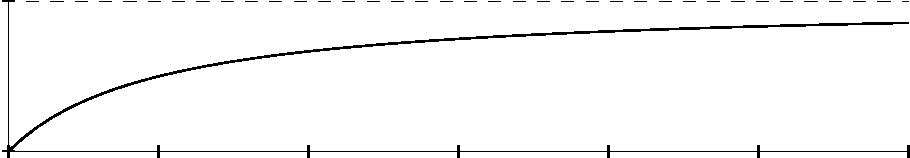
\includegraphics{figures/tovertp1graph}
\caption{Graph of $\frac{t}{t+1}$ for positive $t$ with an asymptote at 1.\label{fig:tovertp1}}
\end{myfigureht}
\end{example}

An important metric space is the
$n$-dimensional \emph{\myindex{euclidean space}}
\glsadd{not:euclidspace}
$\R^n = \R \times \R \times \cdots \times \R$.   We use the following
notation for points: $x =(x_1,x_2,\ldots,x_n) \in \R^n$.  We will not write
$\vec{x}$ nor $\mathbf{x}$ for a point in $\R^n$ as is common in
multivariable calculus,
we simply give it a name such as $x$ and we will remember that $x$
is an element of $\R^n$.
We also
write simply $0 \in \R^n$ to mean the point $(0,0,\ldots,0)$.  Before
making $\R^n$ a metric space, we prove an important inequality, the
so-called Cauchy--Schwarz inequality.

\begin{lemma}[\myindex{Cauchy--Schwarz inequality}%
\footnote{%
Sometimes it is called the \myindex{Cauchy--Bunyakovsky--Schwarz inequality}.
\href{https://en.wikipedia.org/wiki/Hermann_Schwarz}{Karl Hermann Amandus
Schwarz} (1843--1921) was a German mathematician and
\href{https://en.wikipedia.org/wiki/Viktor_Bunyakovsky}{Viktor Yakovlevich
Bunyakovsky} (1804--1889) was a Ukrainian mathematician.  What we
stated should really be called the Cauchy inequality, as
Bunyakovsky and Schwarz provided proofs for infinite-dimensional versions.}]
Suppose $x =(x_1,x_2,\ldots,x_n) \in \R^n$, $y =(y_1,y_2,\ldots,y_n) \in \R^n$.
Then
\begin{equation*}
{\biggl( \sum_{k=1}^n x_k y_k \biggr)}^2
\leq
\biggl(\sum_{k=1}^n x_k^2 \biggr)
\biggl(\sum_{k=1}^n y_k^2 \biggr) .
\end{equation*}
\end{lemma}

\begin{proof}
A square of a real number is nonnegative.  Hence a sum of squares is
nonnegative:
\begin{equation*}
\begin{split}
0 & \leq 
\sum_{k=1}^n \sum_{\ell=1}^n {(x_k y_\ell - x_\ell y_k)}^2
\\
& =
\sum_{k=1}^n \sum_{\ell=1}^n \bigl( x_k^2 y_\ell^2 + x_\ell^2 y_k^2 - 2 x_k
x_\ell y_k
y_\ell \bigr)
\\
& =
\biggl( \sum_{k=1}^n x_k^2 \biggr)
\biggl( \sum_{\ell=1}^n y_\ell^2 \biggr)
+
\biggl( \sum_{k=1}^n y_k^2 \biggr)
\biggl( \sum_{\ell=1}^n x_\ell^2 \biggr)
-
2
\biggl( \sum_{k=1}^n x_k y_k \biggr)
\biggl( \sum_{\ell=1}^n x_\ell y_\ell \biggr) .
\end{split}
\end{equation*}
We relabel and divide by 2 to obtain precisely what we wanted,
\begin{equation*}
0 \leq 
\biggl( \sum_{k=1}^n x_k^2 \biggr)
\biggl( \sum_{k=1}^n y_k^2 \biggr)
-
{\biggl( \sum_{k=1}^n x_k y_k \biggr)}^2 .
\qedhere
\end{equation*}
\end{proof}

\begin{example}
Let us construct the
standard metric\index{standard metric on $\R^n$} for $\R^n$.  Define
\begin{equation*}
d(x,y) \coloneqq
\sqrt{
{(x_1-y_1)}^2 + 
{(x_2-y_2)}^2 + 
\cdots +
{(x_n-y_n)}^2
} =
\sqrt{
\sum_{k=1}^n
{(x_k-y_k)}^2 
} .
\end{equation*}
For $n=1$, the real line, this metric agrees with what we defined above.
For $n > 1$,
the only tricky part of the definition to check, as before, is the triangle inequality.
It is less messy to work with the square of the metric.  In the
following estimate, note the use of the Cauchy--Schwarz inequality.
\begin{equation*}
\begin{split}
{\bigl(d(x,z)\bigr)}^2 & =
\sum_{k=1}^n
{(x_k-z_k)}^2 
\\
& =
\sum_{k=1}^n
{(x_k-y_k+y_k-z_k)}^2 
\\
& =
\sum_{k=1}^n
\Bigl(
{(x_k-y_k)}^2+{(y_k-z_k)}^2 + 2(x_k-y_k)(y_k-z_k)
\Bigr)
\\
& =
\sum_{k=1}^n
{(x_k-y_k)}^2
+
\sum_{k=1}^n
{(y_k-z_k)}^2 
+
2
\sum_{k=1}^n
(x_k-y_k)(y_k-z_k)
\\
& \leq
\sum_{k=1}^n
{(x_k-y_k)}^2
+
\sum_{k=1}^n
{(y_k-z_k)}^2 
+
2
\sqrt{
\sum_{k=1}^n
{(x_k-y_k)}^2
\sum_{k=1}^n
{(y_k-z_k)}^2
}
\\
& =
{\left(
\sqrt{
\sum_{k=1}^n
{(x_k-y_k)}^2
}
+
\sqrt{
\sum_{k=1}^n
{(y_k-z_k)}^2 
}
\right)}^2
=
{\bigl( d(x,y) + d(y,z) \bigr)}^2 .
\end{split}
\end{equation*}
Because the square root is an increasing function, the
inequality is preserved when we 
take the square root of both sides, and we obtain the triangle inequality.
\end{example}

\begin{example}
The set of complex numbers $\C$ is the set of numbers $z = x+iy$, where $x$
and $y$ are in $\R$.  By imposing $i^2 = -1$, we make $\C$ into a
field.
For the purposes of taking limits,
the set $\C$ is regarded as the metric space $\R^2$, where $z=x+iy \in \C$
corresponds to $(x,y) \in \R^2$.
For $z=x+iy$ define the \emph{\myindex{complex modulus}}\index{modulus}
by $\sabs{z} \coloneqq \sqrt{x^2+y^2}$.
Then for two complex numbers
$z_1 = x_1 + iy_1$ and $z_2 = x_2 + iy_2$, the distance is
\begin{equation*}
d(z_1,z_2) = \sqrt{{(x_1-x_2)}^2+ {(y_1-y_2)}^2} = \sabs{z_1-z_2}.
\end{equation*}
Furthermore, when working with complex numbers
it is often convenient to write the metric in terms of
the so-called
\emph{\myindex{complex conjugate}}: The conjugate of $z=x+iy$
is $\bar{z} \coloneqq x-iy$.  Then 
${\sabs{z}}^2 = x^2 +y^2 = z\bar{z}$, and so ${\sabs{z_1-z_2}}^2 =
(z_1-z_2)\overline{(z_1-z_2)}$.
\end{example}

\begin{example}
An example to keep in mind is the so-called
\emph{\myindex{discrete metric}}.
For any set $X$, define
\begin{equation*}
d(x,y) \coloneqq
\begin{cases}
1 & \text{if } x \not= y, \\
0 & \text{if } x = y.
\end{cases}
\end{equation*}
That is, all points are equally distant from each other.  When $X$ is a
finite set, we can draw a diagram, see for example
\figureref{fig:msdiscmetric}.  Of course, in the diagram the distances 
are not the normal euclidean distances in the plane.
Things become subtle when $X$ is an infinite set such
as the real numbers.
\begin{myfigureht}
\subimport*{figures/}{msdiscmetric.pdf_t}
\caption{Sample discrete metric space $\{ a,b,c,d,e \}$, the distance
between any two points is $1$.\label{fig:msdiscmetric}}
\end{myfigureht}

While this particular
example may seldom come up in practice, it gives a useful 
\myquote{smell test.}  If you make a statement about metric spaces,
try it with the discrete metric.
To show that $(X,d)$ is indeed a metric space is left as an exercise.
\end{example}

\begin{example} \label{example:msC01}
Let $C\bigl([a,b],\R\bigr)$\glsadd{not:contfuncs} be the set of
continuous real-valued functions on the interval $[a,b]$.
Define the metric on $C\bigl([a,b],\R\bigr)$ as
\begin{equation*}
d(f,g) \coloneqq \sup_{x \in [a,b]} \abs{f(x)-g(x)} .
\end{equation*}
Let us check the properties.  First, $d(f,g)$ is finite as
$\abs{f(x)-g(x)}$ is a continuous function on a closed bounded interval
$[a,b]$, and so is bounded.
It is clear that $d(f,g) \geq 0$, 
it is the supremum of nonnegative numbers.  If $f = g$,
then $\abs{f(x)-g(x)} = 0$ for all $x$, and hence $d(f,g) = 0$.  Conversely,
if $d(f,g) = 0$, then for every $x$, we have $\abs{f(x)-g(x)} \leq d(f,g) = 0$,
and hence $f(x) = g(x)$ for all $x$, and so $f=g$.  That $d(f,g) = d(g,f)$
is equally trivial.  To show the triangle inequality we use the standard
triangle inequality;
\begin{equation*}
\begin{split}
d(f,g) & =
\sup_{x \in [a,b]} \abs{f(x)-g(x)} =
\sup_{x \in [a,b]} \abs{f(x)-h(x)+h(x)-g(x)}
\\
& \leq
\sup_{x \in [a,b]} \bigl( \abs{f(x)-h(x)}+\abs{h(x)-g(x)} \bigr)
\\
& \leq
\sup_{x \in [a,b]} \abs{f(x)-h(x)}+
\sup_{x \in [a,b]} \abs{h(x)-g(x)} = d(f,h) + d(h,g) .
\end{split}
\end{equation*}
When treating $C\bigl([a,b],\R\bigr)$ as a metric space without mentioning a metric,
we mean this particular metric.
Notice that $d(f,g) = \norm{f-g}_{[a,b]}$, the uniform norm of \defnref{def:unifnorm}.

This example may seem esoteric at first, but it turns out that working with
spaces such as $C\bigl([a,b],\R\bigr)$ is really the meat of a large part of modern 
analysis.  Treating sets of functions as metric spaces allows us to
abstract away a lot of the grubby detail and prove powerful results such as
\hyperref[thm:fs:picard]{Picard's theorem} with less work.
\end{example}

\begin{example}
Another useful example of a metric space is the sphere
with a metric usually called the \emph{\myindex{great circle distance}}.
Let $S^2$ be the \myindex{unit sphere}\index{sphere} in $\R^3$,
that is $S^2 \coloneqq \{ x \in \R^3 : x_1^2+x_2^2+x_3^2 = 1 \}$.
Take $x$ and $y$ in $S^2$, draw a line through the origin and $x$,
and another line through the origin and $y$,
and let $\theta$ be the angle that the two lines make.
Then define $d(x,y) \coloneqq \theta$.  See \figureref{fig:spheremetric}.
The law of cosines from vector calculus says
$d(x,y) = \arccos(x_1y_1+x_2y_2+x_3y_3)$.
It is relatively easy to see that this function satisfies the first three
properties of a metric.
Triangle inequality is harder to prove, and requires a bit more
trigonometry and linear algebra than we wish to indulge in right now, so let
us leave it without proof.

\begin{myfigureht}
\subimport*{figures/}{spheremetric.pdf_t}
\caption{The great circle distance on the unit
sphere.\label{fig:spheremetric}}
\end{myfigureht}

This distance is the shortest distance between points on a sphere if
we are allowed to travel on the sphere only.  It is easy to
generalize to arbitrary diameters.  If we take a sphere of radius
$r$, we let the distance be $d(x,y) \coloneqq r \theta$.  As an example, this is the
standard distance you would use if you compute a distance on the
surface of the earth, such as computing the distance a plane travels from London to
Los Angeles.
\end{example}

Oftentimes it is useful to consider a subset of a larger metric space
as a metric space itself.  We obtain the following proposition, which has
a trivial proof.

\begin{prop}
Let $(X,d)$ be a metric space and $Y \subset X$.  Then the restriction
$d|_{Y \times Y}$ is a metric on $Y$.
\end{prop}

\begin{defn}
If $(X,d)$ is a metric space, $Y \subset X$, and $d' \coloneqq d|_{Y \times Y}$,
then $(Y,d')$ is said to be a \emph{\myindex{subspace}} of $(X,d)$.
\end{defn}

It is common to simply write $d$ for the metric on $Y$, as it is 
the restriction of the metric on $X$.  Sometimes we say $d'$ is
the \emph{\myindex{subspace metric}} and $Y$ has the
\emph{\myindex{subspace topology}}.

\medskip

A subset of the real
numbers is bounded whenever all its elements are at most some fixed distance
from 0.
When dealing with an arbitrary metric space there may not be some
natural fixed point 0, but for the purposes of boundedness it does not matter.

\begin{defn}
Let $(X,d)$ be a metric space.  A subset $S \subset X$ is said to be
\emph{bounded}\index{bounded set} if there exists a $p \in X$ and a
$B \in \R$ such that
\begin{equation*}
d(p,x) \leq B \quad \text{for all } x \in S.
\end{equation*}
We say $(X,d)$ is bounded if $X$ itself is a bounded subset.
\end{defn}

For example, the set of real numbers with the standard metric is not a
bounded metric space.  It is not hard to see that a
subset of the real numbers is bounded in the
sense of \chapterref{rn:chapter} if and only if it is bounded as a subset of the
metric space of real numbers with the standard metric.

On the other hand, if we take the real numbers with the discrete metric,
then we obtain a bounded metric space.  In fact, any set with the
discrete metric is bounded.

There are other equivalent ways we could generalize boundedness,
and are left as exercises.  Suppose $X$ is nonempty to avoid a technicality.
Then $S \subset X$ being bounded is equivalent to either
\begin{enumerate}[(i)]
\item
For every $p \in X$, there exists a $B > 0$ such that $d(p,x) \leq B$ for
all $x \in S$.
\item
\glsadd{not:diam}%
$\operatorname{diam}(S) \coloneqq \sup \bigl\{ d(x,y) : x,y \in S \bigr\} < \infty$.
\end{enumerate}
The quantity $\operatorname{diam}(S)$ is called the
\emph{\myindex{diameter}} of a set and is usually only defined for
a nonempty set.

\subsection{Exercises}

\begin{exercise}
Show that for every set $X$, the discrete metric ($d(x,y) = 1$ if $x\not=y$ and
$d(x,x) = 0$) does give a metric space $(X,d)$.
\end{exercise}

\begin{exercise}
Let $X \coloneqq \{ 0 \}$ be a set.  Can you make it into a metric space?
\end{exercise}

\begin{exercise}
Let $X \coloneqq \{ a, b \}$ be a set.  Can you make it into two distinct metric
spaces?  (define two distinct metrics on it)
\end{exercise}

\begin{exercise}
Let the set $X \coloneqq \{ A, B, C \}$ represent 3 buildings on campus.  Suppose we
wish our distance to be the time it takes to walk from one building to
the other.
It takes 5 minutes either way between buildings $A$ and $B$.  However,
building $C$ is on a hill and it takes 10 minutes from $A$ and 15 minutes
from $B$ to get to $C$.  On the other hand it takes 5 minutes to go
from $C$ to $A$ and 7 minutes to go from $C$ to $B$, as we are going
downhill.  Do these distances define a metric?  If so, prove it, if not, say
why not.
\end{exercise}

\begin{exercise}
Suppose $(X,d)$ is a metric space and
$\varphi \colon [0,\infty) \to \R$ is
an increasing function such that 
$\varphi(t) \geq 0$ for all $t$ and $\varphi(t) = 0$ if and only if
$t=0$.  Also suppose $\varphi$ is \emph{\myindex{subadditive}},
that is, $\varphi(s+t) \leq \varphi(s)+\varphi(t)$.
Show that with $d'(x,y) \coloneqq \varphi\bigl(d(x,y)\bigr)$, we obtain a new
metric space $(X,d')$.
\end{exercise}

\begin{exercise} \label{exercise:mscross}
Let $(X,d_X)$ and $(Y,d_Y)$ be metric spaces.
\begin{enumerate}[a)]
\item
Show that $(X \times Y,d)$ with
$d\bigl( (x_1,y_1), (x_2,y_2) \bigr) \coloneqq d_X(x_1,x_2) + d_Y(y_1,y_2)$ is
a metric space.
\item
Show that $(X \times Y,d)$ with
$d\bigl( (x_1,y_1), (x_2,y_2) \bigr) \coloneqq \max \bigl\{ d_X(x_1,x_2) ,
d_Y(y_1,y_2) \bigr\}$ is
a metric space.
\end{enumerate}
\end{exercise}

\begin{exercise}
Let $X$ be the set of continuous functions on $[0,1]$.  Let $\varphi \colon
[0,1] \to (0,\infty)$ be continuous.  Define
\begin{equation*}
d(f,g) \coloneqq \int_0^1 \abs{f(x)-g(x)}\varphi(x)\,dx .
\end{equation*}
Show that $(X,d)$ is a metric space.
\end{exercise}

\begin{exercise} \label{exercise:mshausdorffpseudo}
Let $(X,d)$ be a metric space.  For nonempty bounded subsets $A$ and $B$ let
\begin{equation*}
d(x,B) \coloneqq \inf \bigl\{ d(x,b) : b \in B \bigl\}
\qquad \text{and} \qquad
d(A,B) \coloneqq \sup \bigl\{ d(a,B) : a \in A \bigr\} .
\end{equation*}
Now define the \emph{\myindex{Hausdorff metric}} as
\begin{equation*}
d_H(A,B) \coloneqq \max \bigl\{ d(A,B) , d(B,A) \bigr\} .
\end{equation*}
Note: $d_H$ can be defined for arbitrary nonempty subsets if we allow the
extended reals.
\begin{enumerate}[a)]
\item
Let $Y \subset \sP(X)$ be the set of bounded nonempty subsets.
Prove that
$(Y,d_H)$ is a so-called \emph{\myindex{pseudometric space}}:
$d_H$ satisfies the metric properties
\ref{metric:pos},
\ref{metric:com}, 
\ref{metric:triang}, and further
$d_H(A,A) = 0$ for all $A \in Y$. 
\item
Show by example that $d$ itself is not symmetric, that is $d(A,B) \not=
d(B,A)$.
\item
Find a metric space $X$ and two different
nonempty bounded subsets $A$ and $B$ such that $d_H(A,B) = 0$.
\end{enumerate}
\end{exercise}

\begin{exercise}
Let $(X,d)$ be a nonempty metric space and $S \subset X$ a subset.  Prove:
\begin{enumerate}[a)]
\item
$S$ is bounded if and only if
for every $p \in X$, there exists a $B > 0$ such that $d(p,x) \leq B$ for
all $x \in S$.
\item
A nonempty $S$ is bounded if and only if
$\operatorname{diam}(S) \coloneqq \sup \{ d(x,y) : x,y \in S \} < \infty$.
\end{enumerate}
\end{exercise}

\begin{exercise}
\pagebreak[2]
\leavevmode
\begin{enumerate}[a)]
\item
Working in $\R$, compute $\operatorname{diam}\bigl([a,b]\bigr)$.
\item
Working in $\R^n$, for every $r > 0$, let $B_r \coloneqq \{ x_1^2+x_2^2+\cdots+x_n^2
< r^2 \}$.  Compute $\operatorname{diam}(B_r)$.
\item
Suppose $(X,d)$ is a metric space with at least two points,
$d$ is the discrete metric, and $p \in X$.
Compute
$\operatorname{diam}(\{ p \})$ and $\operatorname{diam}(X)$,
then conclude that $(X,d)$ is bounded.
\end{enumerate}
\end{exercise}

\begin{exercise}
\pagebreak[2]
\leavevmode
\begin{enumerate}[a)]
\item
Find a metric $d$ on $\N$ such that $\N$ is an unbounded set in $(\N,d)$.
\item
Find a metric $d$ on $\N$ such that $\N$ is a bounded set in $(\N,d)$.
\item
Find a metric $d$ on $\N$ such that for every $n \in \N$ and every $\epsilon > 0$,
there exists an $m \in \N$ such that $d(n,m) < \epsilon$.
\end{enumerate}
\end{exercise}

\begin{exercise} \label{exercise:C1ab}
Let $C^1\bigl([a,b],\R\bigr)$\glsadd{not:contdifffuncs} be the set of once continuously differentiable
functions on $[a,b]$.
Define
\begin{equation*}
d(f,g) \coloneqq \snorm{f-g}_{[a,b]} + \snorm{f'-g'}_{[a,b]},
\end{equation*}
where $\snorm{\cdot}_{[a,b]}$ is the uniform norm.  Prove that $d$ is a metric.
\end{exercise}

\begin{samepage}
\begin{exercise}
Consider $\ell^2$ the set of sequences $\{ x_n \}_{n=1}^\infty$
of real numbers
such that $\sum_{n=1}^\infty x_n^2 < \infty$.
\begin{enumerate}[a)]
\item
Prove the \myindex{Cauchy--Schwarz inequality} for two sequences
$\{x_n \}_{n=1}^\infty$ and $\{ y_n \}_{n=1}^\infty$ in $\ell^2$:  Prove that
$\sum_{n=1}^\infty x_n y_n$ converges (absolutely) and
\begin{equation*}
{\biggl( \sum_{n=1}^\infty x_n y_n \biggr)}^2
\leq
\biggl(\sum_{n=1}^\infty x_n^2 \biggr)
\biggl(\sum_{n=1}^\infty y_n^2 \biggr) .
\end{equation*}
\item
Prove that $\ell^2$ is a metric space with the metric
$d(x,y) \coloneqq \sqrt{\sum_{n=1}^\infty {(x_n-y_n)}^2}$.
Hint: Don't forget to show that the series for $d(x,y)$ always converges
to some finite number.
\end{enumerate}
\end{exercise}
\end{samepage}

%%%%%%%%%%%%%%%%%%%%%%%%%%%%%%%%%%%%%%%%%%%%%%%%%%%%%%%%%%%%%%%%%%%%%%%%%%%%%%

\sectionnewpage
\section{Open and closed sets}
\label{sec:mettop}

%mbxINTROSUBSECTION

\sectionnotes{2 lectures}

\subsection{Topology}

Before we get to convergence,
we define the so-called \emph{\myindex{topology}}.
That is,
we define open and closed sets in a metric space.
And before that,
we define two special open and closed sets.

\begin{defn}
Let $(X,d)$ be a metric space, $x \in X$, and $\delta > 0$.  Define
the \emph{\myindex{open ball}}, or simply \emph{\myindex{ball}}, of radius $\delta$
around $x$ as
\glsadd{not:openball}
\begin{equation*}
B(x,\delta) \coloneqq \bigl\{ y \in X : d(x,y) < \delta \bigr\} .
\end{equation*}
Define the \emph{\myindex{closed ball}} as
\glsadd{not:closedball}
\begin{equation*}
C(x,\delta) \coloneqq \bigl\{ y \in X : d(x,y) \leq \delta \bigr\} .
\end{equation*}
\end{defn}

When dealing with different metric spaces, it is sometimes 
vital to emphasize which metric space the ball is in.  We do this by
writing $B_X(x,\delta) \coloneqq B(x,\delta)$ or $C_X(x,\delta) \coloneqq C(x,\delta)$.

\begin{example}
Take the metric space $\R$ with the standard metric.  For
$x \in \R$ and $\delta > 0$,
\begin{equation*}
B(x,\delta) = (x-\delta,x+\delta) \qquad \text{and} \qquad
C(x,\delta) = [x-\delta,x+\delta] .
\end{equation*}
\end{example}

\begin{example}
Be careful when working on a subspace.  Consider the
metric space $[0,1]$ as a subspace of $\R$.  Then in $[0,1]$,
\begin{equation*}
B(0,\nicefrac{1}{2}) = B_{[0,1]}(0,\nicefrac{1}{2})
= \bigl\{ y \in [0,1] : \abs{0-y} < \nicefrac{1}{2} \bigr\}
= [0,\nicefrac{1}{2}) .
\end{equation*}
This is different from $B_{\R}(0,\nicefrac{1}{2}) =
(\nicefrac{-1}{2},\nicefrac{1}{2})$.
The important thing to keep in mind is which metric space we are working
in.
\end{example}

\begin{defn}
Let $(X,d)$ be a metric space.  A subset $V \subset X$
is \emph{open}\index{open set}
if for every $x \in V$, there exists a $\delta > 0$ such that
$B(x,\delta) \subset V$.  See \figureref{fig:msopenset}.  A subset $E \subset X$ is 
\emph{closed}\index{closed set} if the complement $E^c = X \setminus E$ is open.
When the ambient space $X$ is not clear from context,
we say \emph{$V$ is open in $X$} and \emph{$E$ is closed in $X$}.

If $x \in V$ and $V$ is open, then we say 
$V$ is an \emph{\myindex{open neighborhood}} of $x$ (or
sometimes just \emph{\myindex{neighborhood}}).
\end{defn}

\begin{myfigureht}
\subimport*{figures/}{msopenset.pdf_t}
\caption{Open set in a metric space.  Note that $\delta$ depends on $x$.\label{fig:msopenset}}
\end{myfigureht}

Intuitively, an open set $V$ is a set that does not include its
\myquote{boundary.}
Wherever we are in $V$,
we are allowed to \myquote{wiggle} a little bit and
stay in $V$.  Similarly, a set $E$ is closed if everything not in $E$
is some distance away from $E$.
The open and closed balls are examples of open and closed sets
(this must still be proved).
But not every set is either open or closed.  Generally, most subsets are neither.

\begin{example}
The set $(0,\infty) \subset \R$ is open:  Given any $x \in (0,\infty)$,
let $\delta \coloneqq x$.  Then $B(x,\delta) = (0,2x) \subset (0,\infty)$.

The set $[0,\infty) \subset \R$ is closed:  Given $x \in (-\infty,0) =
[0,\infty)^c$,
let $\delta \coloneqq -x$.  Then $B(x,\delta) = (-2x,0) \subset
(-\infty,0) = [0,\infty)^c$.

The set $[0,1) \subset \R$ is neither open nor closed.  First,
every ball in $\R$ around $0$, $B(0,\delta) = (-\delta,\delta)$, contains negative
numbers and hence is not contained in $[0,1)$.  So $[0,1)$ is not open.
Second, every ball in $\R$ around $1$,
$B(1,\delta) = (1-\delta,1+\delta)$, contains
numbers strictly less than 1 and greater than 0
(e.g.\ $1-\nicefrac{\delta}{2}$ as long as $\delta < 2$).
Thus $[0,1)^c = \R \setminus
[0,1)$ is not open, and $[0,1)$ is not closed.

If $(X,d)$ is any metric space, and $x \in X$ is a point, then $\{ x \}$ is
closed (exercise).
On the other hand, $\{ x \}$ may or may not be open depending on $X$.
The set $\{ 0 \} \subset \R$ is not open as $B(0,\delta)$
contains nonzero numbers for every $\delta > 0$.
If $X=\{ x \}$, then $\{ x \}$ is open.
\end{example}

\begin{prop} \label{prop:topology:open}
Let $(X,d)$ be a metric space.
\begin{enumerate}[(i)]
\item \label{topology:openi} $\emptyset$ and $X$ are open.
\item \label{topology:openii} If $V_1, V_2, \ldots, V_k$ are open subsets of $X$, then
\begin{equation*}
\bigcap_{j=1}^k V_j
\end{equation*}
is also open.  That is, a finite intersection of open sets is open.
\item \label{topology:openiii} If $\{ V_\lambda \}_{\lambda \in I}$ is
an arbitrary collection of open subsets of $X$, then
\begin{equation*}
\bigcup_{\lambda \in I} V_\lambda
\end{equation*}
is also open.  That is, a union of open sets is open.
\end{enumerate}
\end{prop}

The index set $I$ in \ref{topology:openiii} can be arbitrarily large.
By $\bigcup_{\lambda \in I} V_\lambda$, we simply mean the set of
all~$x$ such that $x \in V_\lambda$ for at least one $\lambda \in I$.

\begin{proof}
The sets $\emptyset$ and $X$ are obviously open in $X$.

Let us prove \ref{topology:openii}.
If $x \in \bigcap_{j=1}^k V_j$, then $x \in V_j$ for all $j$.
As $V_j$ are all open, for every $j$ there exists a $\delta_j > 0$ 
such that $B(x,\delta_j) \subset V_j$.  Take $\delta \coloneqq \min \{
\delta_1,\delta_2,\ldots,\delta_k \}$ and notice $\delta > 0$.  We have
$B(x,\delta) \subset B(x,\delta_j) \subset V_j$ for every $j$ and so
$B(x,\delta) \subset \bigcap_{j=1}^k V_j$.  Consequently the intersection is open.

Let us prove \ref{topology:openiii}.
If $x \in \bigcup_{\lambda \in I} V_\lambda$, then $x \in V_\lambda$ for some
$\lambda \in I$.
As $V_\lambda$ is open, there exists a $\delta > 0$
such that $B(x,\delta) \subset V_\lambda$.  But then
$B(x,\delta) \subset \bigcup_{\lambda \in I} V_\lambda$,
and so the union is open.
\end{proof}

\begin{example}
Notice the difference between
items
\ref{topology:openii} and \ref{topology:openiii}.
Item \ref{topology:openii} is not true for an arbitrary intersection.
For instance,
$\bigcap_{n=1}^\infty (\nicefrac{-1}{n},\nicefrac{1}{n}) = \{ 0 \}$,
which is not open.
\end{example}


The proof of the following analogous proposition for closed sets
is left as an exercise.

\begin{prop} \label{prop:topology:closed}
%FIXMEevillayouthack
\pagebreak[2]
Let $(X,d)$ be a metric space.
\begin{enumerate}[(i)]
\item \label{topology:closedi} $\emptyset$ and $X$ are closed.
\item \label{topology:closedii} If $\{ E_\lambda \}_{\lambda \in I}$ is
an arbitrary collection of closed subsets of $X$, then
\begin{equation*}
\bigcap_{\lambda \in I} E_\lambda
\end{equation*}
is also closed.  That is, an intersection of closed sets is closed.
\item \label{topology:closediii} If $E_1, E_2, \ldots, E_k$ are closed
subsets of $X$, then
\begin{equation*}
\bigcup_{j=1}^k E_j
\end{equation*}
is also closed.  That is, a finite union of closed sets is closed.
\end{enumerate}
\end{prop}

Despite the naming,
we have not yet shown that the open ball is open and the closed ball is
closed.  Let us show these facts now to justify the terminology.

\begin{prop} \label{prop:topology:ballsopenclosed}
Let $(X,d)$ be a metric space, $x \in X$, and $\delta > 0$.  Then
$B(x,\delta)$ is open and 
$C(x,\delta)$ is closed.
\end{prop}

\begin{proof}
Let $y \in B(x,\delta)$.  Let $\alpha \coloneqq \delta-d(x,y)$.  As $\alpha
> 0$, consider $z \in B(y,\alpha)$.  Then
\begin{equation*}
d(x,z) \leq d(x,y) + d(y,z) < d(x,y) + \alpha = d(x,y) + \delta-d(x,y) =
\delta .
\end{equation*}
Therefore, $z \in B(x,\delta)$ for every $z \in B(y,\alpha)$.  So
$B(y,\alpha) \subset B(x,\delta)$, and so
$B(x,\delta)$ is open.  See \figureref{fig:ballisopen}.

\begin{myfigureht}
\subimport*{figures/}{ballisopen.pdf_t}
\caption{Proof that $B(x,\delta)$ is open: $B(y,\alpha) \subset
B(x,\delta)$ with the triangle inequality illustrated.\label{fig:ballisopen}}
\end{myfigureht}

The proof that $C(x,\delta)$ is closed is left as an exercise.
\end{proof}

Again, be careful about which metric space we are in.
The set $[0,\nicefrac{1}{2})$ is
an open ball in $[0,1]$, and so $[0,\nicefrac{1}{2})$ is
an open set in $[0,1]$.  On the other hand, $[0,\nicefrac{1}{2})$
is neither open nor closed in $\R$.

\begin{prop} \label{prop:topology:intervals:openclosed}
Let $a, b$ be two real numbers, $a < b$.  Then $(a,b)$, $(a,\infty)$,
and $(-\infty,b)$ are open in $\R$.
Also $[a,b]$, $[a,\infty)$,
and $(-\infty,b]$ are closed in $\R$.
\end{prop}

The proof is left as an exercise.  Keep in mind that
there are many other open and
closed sets in the set of real numbers. %$\R$.

\begin{prop} \label{prop:topology:subspaceopen}
Suppose $(X,d)$ is a metric space, and $Y \subset X$.  Then $U \subset Y$
is open in $Y$ (in the subspace topology) if and only if
there exists an open set $V \subset X$ (so open in $X$) such that
$V \cap Y = U$.
\end{prop}

For example, let $X \coloneqq \R$, $Y \coloneqq [0,1]$, $U \coloneqq [0,\nicefrac{1}{2})$.
We saw that $U$ is an open set in $Y$.
We may take $V \coloneqq (\nicefrac{-1}{2},\nicefrac{1}{2})$.

\begin{proof}
Suppose $V \subset X$ is open and $V \cap Y = U$.
Let $x \in U$.
As $V$ is open and $x \in V$, there
exists a $\delta > 0$ such that $B_X(x,\delta) \subset V$.
Then
\begin{equation*}
B_Y(x,\delta) = B_X(x,\delta) \cap Y \subset V \cap Y = U .
\end{equation*}
So $U$ is open in $Y$.

The proof of the opposite direction, that is, that if $U \subset Y$
is open in the subspace topology there exists a $V$ is left as
\exerciseref{exercise:mssubspace}.
\end{proof}

A hint for finishing the proof (the exercise) is that
a useful way to think about an open set is as a union of open balls.  If $U$ is
open, then for each $x \in U$, there is a $\delta_x > 0$ (depending on $x$) such that
$B(x,\delta_x) \subset U$.  Then $U = \bigcup_{x\in U} B(x,\delta_x)$.

In the case of an open subset of an open set or a closed subset of a closed
set, matters are simpler.

\begin{prop} \label{prop:topology:subspacesame}
Suppose $(X,d)$ is a metric space, $V \subset X$ is open,
and $E \subset X$ is closed.
\begin{enumerate}[(i)]
\item \label{prop:topology:subspacesame:i}
$U \subset V$ is open in the subspace topology if and only if $U$ is open
in $X$.
\item \label{prop:topology:subspacesame:ii}
$F \subset E$ is closed in the subspace topology if and only if $F$ is
closed in $X$.
\end{enumerate}
\end{prop}

\begin{proof}
We prove
\ref{prop:topology:subspacesame:i}
and leave 
\ref{prop:topology:subspacesame:ii} as an exercise.

If $U \subset V$ is open in the subspace topology, by
\propref{prop:topology:subspaceopen}, there is a set $W \subset X$
open in $X$ such that $U = W \cap V$.  Intersection of two open sets
is open so $U$ is open in $X$.

Now suppose $U$ is open in $X$.  Then $U = U \cap V$. So
$U$ is open in $V$ again by \propref{prop:topology:subspaceopen}.
\end{proof}

\subsection{Connected sets}

Let us generalize the idea of an interval to general metric spaces.  One of
the main features of an interval in $\R$ is that it is
connected---that we can continuously move from one point of it to
another point without jumping.
For example, in $\R$ we usually study functions on intervals,
and in more general metric spaces we usually study functions on connected sets.

\begin{defn}
A nonempty%
\footnote{Some authors do not exclude the empty set from the definition,
and the empty set would then be connected.
We avoid the empty set for essentially the same reason why
1 is neither a prime nor a composite number:  Our connected sets have exactly
two clopen subsets and disconnected sets have more than two.  The empty set
has exactly one.}
metric space $(X,d)$ is \emph{\myindex{connected}} if the
only subsets of $X$ that are both open and closed (so-called
\emph{\myindex{clopen}} subsets) are $\emptyset$ and $X$ itself.
If a nonempty $(X,d)$ is not connected we say it is
\emph{\myindex{disconnected}}.

When we apply the term \emph{connected} to a nonempty subset $A \subset X$, we 
mean that $A$ with the subspace topology is connected.
\end{defn}

In other words, a nonempty $X$ is connected if whenever we write
$X = X_1 \cup X_2$ where $X_1 \cap X_2 = \emptyset$ and $X_1$ and $X_2$ are
open, then either $X_1 = \emptyset$ or $X_2 = \emptyset$.
So to show $X$ is disconnected, we need to find nonempty
disjoint open sets $X_1$ and
$X_2$ whose union is $X$.
For subsets, we state this idea as a proposition.
The proposition is illustrated in \figureref{fig:disconsubset}.

\begin{prop}
Let $(X,d)$ be a metric space.
A nonempty set $S \subset X$ is disconnected if and only if
there exist open sets $U_1$ and
$U_2$ in $X$ such that $U_1 \cap U_2 \cap S = \emptyset$,
$U_1 \cap S \not= \emptyset$,
$U_2 \cap S \not= \emptyset$, and
\begin{equation*}
S = 
\bigl( U_1 \cap S \bigr)
\cup
\bigl( U_2 \cap S \bigr) .
\end{equation*}
\end{prop}

\begin{myfigureht}
\subimport*{figures/}{disconsubset.pdf_t}
\caption{Disconnected subset.  Notice that $U_1 \cap U_2$ need
not be empty, but $U_1 \cap U_2 \cap S = \emptyset$.\label{fig:disconsubset}}
\end{myfigureht}


\begin{proof}
First suppose $S$ is disconnected: There are
nonempty disjoint $S_1$ and $S_2$ that are
open in $S$ and $S = S_1 \cup S_2$.
\propref{prop:topology:subspaceopen} says there exist $U_1$ and $U_2$
that are open in $X$ such that $U_1 \cap S = S_1$ and
$U_2 \cap S = S_2$.

For the other direction start with the $U_1$ and $U_2$.
Then $U_1 \cap S$ and $U_2 \cap S$ are open in $S$ by
\propref{prop:topology:subspaceopen}.
Via the discussion before the proposition, $S$ is disconnected.
\end{proof}

\begin{example}
Suppose $S \subset \R$ and there are $x,y,z$ such that $x < z < y$ with $x,y \in S$
and $z \notin S$.  Claim: \emph{$S$ is disconnected}.  Proof:  Notice
\begin{equation*}
\bigl( (-\infty,z) \cap S \bigr)
\cup
\bigl( (z,\infty) \cap S \bigr)
= S .
\end{equation*}
\end{example}

\begin{prop}
A nonempty set $S \subset \R$ is connected if and only if $S$ is
an interval or a single point.
\end{prop}

\begin{proof}
Suppose $S$ is connected.  If $S$ is a single point,
then we are done.  So suppose $x < y$ and $x,y \in S$.  If $z \in \R$ is such
that $x < z < y$, then $(-\infty,z) \cap S$ is nonempty and $(z,\infty) \cap
S$ is nonempty.  The two sets are disjoint.  As
$S$ is connected, we must have they their union is not $S$, so $z \in S$.
By \propref{prop:intervaldef}, $S$ is an interval.

If $S$ is a single point, it is connected.
Therefore, suppose $S$ is an interval.
Consider open subsets $U_1$ and $U_2$ of $\R$ such that
$U_1 \cap S$ and $U_2 \cap S$ are nonempty, and
$S = 
\bigl( U_1 \cap S \bigr)
\cup
\bigl( U_2 \cap S \bigr)$.  We will show that $U_1 \cap S$
and $U_2 \cap S$ contain a common point, so they are not disjoint,
proving that $S$ is connected.
Suppose $x \in U_1 \cap S$
and $y \in U_2 \cap S$.  Without loss of generality, assume $x < y$.
As $S$ is an interval, $[x,y] \subset S$.
Note that $U_2 \cap [x,y] \not= \emptyset$, and
let $z \coloneqq \inf (U_2 \cap [x,y])$.
We wish to show that $z \in U_1$.
If $z = x$, then $z \in U_1$.
If $z > x$,
then for every $\epsilon > 0$, the ball $B(z,\epsilon) =
(z-\epsilon,z+\epsilon)$ contains points of $[x,y]$ not in $U_2$,
as $z$ is the infimum of $U_2 \cap [x,y]$.
So $z \notin U_2$ as $U_2$ is open.
Therefore, $z \in U_1$ as every point of $[x,y]$ is in
$U_1$ or $U_2$.
As $U_1$ is open,
$B(z,\delta) \subset U_1$ for a small enough $\delta > 0$.
As $z$ is the infimum of the nonempty set $U_2 \cap [x,y]$, 
there must exist some $w \in U_2 \cap [x,y]$
such that $w \in [z,z+\delta) \subset B(z,\delta) \subset U_1$.
Therefore, $w \in U_1 \cap U_2 \cap [x,y]$.
So $U_1 \cap S$ and $U_2 \cap S$ are not disjoint, and
$S$ is connected.
See \figureref{fig:intervalcon}.
\end{proof}

\begin{myfigureht}
\subimport*{figures/}{intervalcon.pdf_t}
\caption{Proof that an interval is connected.\label{fig:intervalcon}}
\end{myfigureht}

\begin{example}
Oftentimes a ball $B(x,\delta)$ is connected, but this is not
necessarily true in every metric space.
For a simplest example,
take a two point space $\{ a, b\}$ with the discrete metric.
Then $B(a,2) = \{ a , b \}$, which is not
connected as $B(a,1) = \{ a \}$ and 
$B(b,1) = \{ b \}$ are open and disjoint.
\end{example}

\subsection{Closure and boundary}

Sometimes we wish to take a set and throw in everything that we can approach
from the set.  This concept is called the closure.

\begin{defn}
Let $(X,d)$ be a metric space and $A \subset X$.
The \emph{\myindex{closure}} of $A$ is the set
\glsadd{not:closure}
\begin{equation*}
\widebar{A} \coloneqq \bigcap \{ E \subset X : E \text{ is closed and } A \subset
E \} .
\end{equation*}
\end{defn}

That is,
$\widebar{A}$ is the intersection of all closed sets that contain $A$.


\begin{prop}
Let $(X,d)$ be a metric space and $A \subset X$.  The closure $\widebar{A}$
is closed, and $A \subset \widebar{A}$.
Furthermore, if $A$ is closed, then $\widebar{A} = A$.
\end{prop}

\begin{proof}
The closure is an intersection of closed sets, so $\widebar{A}$ is closed.
There is at least one closed set containing $A$, namely $X$ itself,
so $A \subset \widebar{A}$.
If $A$ is closed, then $A$ is a closed set that contains $A$.
So $\widebar{A} \subset A$, and thus $A = \widebar{A}$.
\end{proof}

\begin{example}
The closure of $(0,1)$ in $\R$ is $[0,1]$.  Proof:  If
$E$ is closed and contains $(0,1)$, then $E$ contains $0$ and $1$ (why?).
Thus $[0,1] \subset E$.  But $[0,1]$ is also closed.
Hence, the closure $\overline{(0,1)} = [0,1]$.
\end{example}

\begin{example}
Be careful to notice what ambient metric space you are working with.
If $X = (0,\infty)$, then
the closure of $(0,1)$ in $(0,\infty)$ is $(0,1]$.  Proof:  Similarly as
above, $(0,1]$ is closed in $(0,\infty)$ (why?).  Any closed set $E$
that contains $(0,1)$ must contain 1 (why?).  Therefore, $(0,1] \subset E$,
and hence $\overline{(0,1)} = (0,1]$ when working in $(0,\infty)$.
\end{example}

Let us justify the statement that the closure is everything that we can
\myquote{approach} from within the set.

\begin{prop} \label{prop:msclosureappr}
Let $(X,d)$ be a metric space and $A \subset X$.  Then $x \in \widebar{A}$
if and only if for every $\delta > 0$, $B(x,\delta) \cap A \not=\emptyset$.
\end{prop}

\begin{proof}
Let us prove the two contrapositives.
Let us show that $x \notin \widebar{A}$ if and only if there exists
a $\delta > 0$ such that $B(x,\delta) \cap A = \emptyset$.

First suppose $x \notin \widebar{A}$.  We know $\widebar{A}$ is
closed.  Thus there is a $\delta > 0$ such that
$B(x,\delta) \subset \widebar{A}^c$.  As $A \subset \widebar{A}$ we
see that $B(x,\delta) \subset \widebar{A}^c \subset A^c$ and hence
$B(x,\delta) \cap A = \emptyset$.

On the other hand, suppose there is a $\delta > 0$ such that
$B(x,\delta) \cap A = \emptyset$. 
In other words,
$A \subset {B(x,\delta)}^c$.
As 
${B(x,\delta)}^c$ is a closed set, as $x \not \in {B(x,\delta)}^c$,
and as $\widebar{A}$ is the intersection
of closed sets containing $A$, we have $x \notin \widebar{A}$.
\end{proof}

We can also talk about the interior of a set
(points we cannot approach from the complement),
and the boundary of a set (points we can
approach both from the set and its complement).

\begin{defn}
Let $(X,d)$ be a metric space and $A \subset X$.
The \emph{\myindex{interior}} of $A$ is the set
\glsadd{not:interior}
\begin{equation*}
A^\circ \coloneqq \{ x \in A : \text{there exists a } \delta > 0
\text{ such that } B(x,\delta) \subset A \} .
\end{equation*}
The \emph{\myindex{boundary}} of $A$ is the set
\glsadd{not:boundary}
\begin{equation*}
\partial A \coloneqq \widebar{A}\setminus A^\circ.
\end{equation*}
\end{defn}

Alternatively, the interior is the union of open sets lying in $A$,
see \exerciseref{exercise:interiortopologic}.  By
definition, $A^\circ \subset A$;
however, the points of the boundary may or may not be in $A$.

\begin{example}
Suppose $A \coloneqq (0,1]$ and $X \coloneqq \R$.  Then $\widebar{A}=[0,1]$, $A^\circ = (0,1)$,
and $\partial A = \{ 0, 1 \}$.
\end{example}

\begin{example}
Consider $X \coloneqq \{ a, b \}$ with the discrete metric,
and let $A \coloneqq \{ a \}$.  Then $\widebar{A} = A^\circ = A$ and $\partial A =
\emptyset$.
\end{example}


\begin{prop}
Let $(X,d)$ be a metric space and $A \subset X$.  Then $A^\circ$ is open
and $\partial A$ is closed.
\end{prop}

\begin{proof}
Given $x \in A^\circ$, there is a $\delta > 0$ such that $B(x,\delta)
\subset A$.  If $z \in B(x,\delta)$, then as open balls are open,
there is an $\epsilon > 0$ such that $B(z,\epsilon) \subset B(x,\delta)
\subset A$.  So $z \in A^\circ$.  Therefore, $B(x,\delta) \subset
A^\circ$, and so $A^\circ$ is open.

As $A^\circ$ is open, then
$\partial A = \widebar{A} \setminus A^\circ = \widebar{A} \cap
{(A^\circ)}^c$ is closed.
\end{proof}

The boundary is the set of points that are close to both the set and its
complement.  See \figureref{fig:msboundary} for a diagram
of the next proposition.

\begin{prop}
Let $(X,d)$ be a metric space and $A \subset X$.  Then $x \in \partial A$
if and only if for every $\delta > 0$,
$B(x,\delta) \cap A$ and
$B(x,\delta) \cap A^c$ are both nonempty.
\end{prop}

\begin{myfigureht}
\subimport*{figures/}{msboundary.pdf_t}
\caption{Boundary is the set where every ball contains points in the set and
also its complement.\label{fig:msboundary}}
\end{myfigureht}

\begin{proof}
Suppose $x \in \partial A =  \widebar{A} \setminus A^\circ$ and
let $\delta > 0$ be arbitrary.
By \propref{prop:msclosureappr}, $B(x,\delta)$ contains
a point of $A$.  If $B(x,\delta)$ contained no points of $A^c$,
then $x$ would be in $A^\circ$.  Hence $B(x,\delta)$ contains a point of
$A^c$ as well.

Let us prove the other direction by contrapositive.  
Suppose $x \notin \partial A$, so $x \notin \widebar{A}$ or $x \in A^\circ$.
If $x \notin \widebar{A}$, then
$B(x,\delta) \subset \widebar{A}^c$
for some $\delta > 0$ as $\widebar{A}$ is closed.
So $B(x,\delta) \cap A$ is empty, because $\widebar{A}^c \subset
A^c$.
If $x \in A^\circ$, then
$B(x,\delta) \subset A$ for some $\delta > 0$,
so $B(x,\delta) \cap A^c$ is empty.
\end{proof}

We obtain the following immediate corollary about closures of $A$ and $A^c$.  We
simply apply \propref{prop:msclosureappr}.

\begin{cor}
Let $(X,d)$ be a metric space and $A \subset X$.
Then $\partial A = \widebar{A} \cap \widebar{A^c}$.
\end{cor}

\subsection{Exercises}

\begin{exercise}
Prove \propref{prop:topology:closed}.  Hint:
Apply \propref{prop:topology:open} to
the complements of the sets.
\end{exercise}

\begin{exercise}
Finish the proof of \propref{prop:topology:ballsopenclosed} by
proving that $C(x,\delta)$ is closed.
\end{exercise}

\begin{exercise}
Prove \propref{prop:topology:intervals:openclosed}.
\end{exercise}

\begin{exercise}
Suppose $(X,d)$ is a nonempty metric space with the discrete topology.  Show
that $X$ is connected if and only if it contains exactly one element.
\end{exercise}

\begin{exercise}
Take $\Q$ with the standard metric, $d(x,y) = \abs{x-y}$, as our metric space.
Prove that $\Q$ is
\emph{\myindex{totally disconnected}}, that is, show 
that for every $x, y \in \Q$ with $x \not= y$, there exists an
two open sets $U$ and $V$ such that $x \in U$, $y \in V$,
$U \cap V = \emptyset$, and $U \cup V = \Q$.
\end{exercise}

\begin{exercise}
Show that in a metric space,
every open set can be written as a union of closed sets.
\end{exercise}

\begin{samepage}
\begin{exercise}
Prove that in a metric space,
\begin{enumerate}[a)]
\item
$E$ is closed if and only if $\partial E \subset E$.
\item
$U$ is open if and only if $\partial U \cap U = \emptyset$.
\end{enumerate}
\end{exercise}
\end{samepage}

\begin{exercise}
Prove that in a metric space,
\begin{enumerate}[a)]
\item
$A$ is open if and only if $A^\circ = A$.
\item
$U \subset A^\circ$
for every open set $U$ such that $U \subset A$.
\end{enumerate}
\end{exercise}

\begin{exercise}
Let $X$ be a set and $d$, $d'$ be two metrics on $X$.
Suppose there exists an $\alpha > 0$ and $\beta > 0$
such that $\alpha d(x,y) \leq d'(x,y) \leq \beta d(x,y)$ for all $x,y \in X$.
Show that $U$ is open in $(X,d)$ if and only if $U$ is open in $(X,d')$.
That is, the topologies of $(X,d)$ and $(X,d')$ are the same.
\end{exercise}


\begin{exercise}
Suppose $\{ S_i \}$, $i \in \N$,
is a collection of connected subsets of a metric space $(X,d)$,
and there exists an $x \in X$ such that $x \in S_i$ for all $i \in \N$.
Show that $\bigcup_{i=1}^\infty S_i$ is connected.
\end{exercise}

\begin{exercise}
\pagebreak[2]
Let $A$ be a connected set in a metric space.
\begin{enumerate}[a)]
\item
Is $\widebar{A}$ connected?  Prove or find a counterexample.
\item
Is $A^\circ$ connected?  Prove or find a counterexample.
\end{enumerate}
Hint: Think of sets in $\R^2$.
\end{exercise}

\begin{exercise} \label{exercise:mssubspace}
Finish the proof of \propref{prop:topology:subspaceopen}.
Suppose $(X,d)$ is a metric space and $Y \subset X$.  Show that
with the subspace metric on $Y$, if a set $U \subset Y$
is open (in $Y$), then there exists an open set $V \subset X$ such
that $U = V \cap Y$.
\end{exercise}

\begin{samepage}
\begin{exercise}
Let $(X,d)$ be a metric space.
\begin{enumerate}[a)]
\item
For every $x \in X$ and $\delta > 0$, show
$\overline{B(x,\delta)} \subset C(x,\delta)$.
\item
Is it always true that
$\overline{B(x,\delta)} = C(x,\delta)$?  Prove or find a counterexample.
\end{enumerate}
\end{exercise}
\end{samepage}

\begin{exercise} \label{exercise:interiortopologic}
Let $(X,d)$ be a metric space and $A \subset X$.  Show that
$A^\circ = \bigcup \{ V : V \text{ is open and } V \subset A \}$.
\end{exercise}

\begin{exercise}
Finish the proof of \propref{prop:topology:subspacesame}.
\end{exercise}

\begin{exercise}
Let $(X,d)$ be a metric space.  Show that there exists a bounded metric
$d'$ such that $(X,d')$ has the same open sets, that is, the topology is
the same.
\end{exercise}

\begin{samepage}
\begin{exercise}
Let $(X,d)$ be a metric space.
\begin{enumerate}[a)]
\item
Prove that for every $x \in X$, there either exists a $\delta > 0$ such that
$B(x,\delta) = \{ x \}$, or $B(x,\delta)$ is infinite for every $\delta >  0$.
\item
Find an explicit example of $(X,d)$, $X$ infinite, where
for every $\delta > 0$ and
every $x \in X$, the
ball $B(x,\delta)$ is finite.
\item
Find an explicit example of $(X,d)$ where for every $\delta > 0$ and
every $x \in X$, the
ball $B(x,\delta)$ is countably infinite.
\item
Prove that if $X$ is uncountable, then there exists
an $x \in X$ and a $\delta > 0$ such that $B(x,\delta)$ is uncountable.
\end{enumerate}
\end{exercise}
\end{samepage}

\begin{exercise}
For every $x \in \R^n$ and every $\delta > 0$ define the \myquote{rectangle}
$R(x,\delta) \coloneqq
(x_1-\delta,x_1+\delta) \times
(x_2-\delta,x_2+\delta) \times \cdots \times
(x_n-\delta,x_n+\delta)$.  Show that these sets generate the same open
sets as the balls in standard metric.  That is, show that a set $U \subset \R^n$
is open in the sense of the standard metric if and only if for every
point $x \in U$, there exists a $\delta > 0$ such that $R(x,\delta) \subset
U$.
\end{exercise}

%%%%%%%%%%%%%%%%%%%%%%%%%%%%%%%%%%%%%%%%%%%%%%%%%%%%%%%%%%%%%%%%%%%%%%%%%%%%%%

\sectionnewpage
\section{Sequences and convergence}
\label{sec:metseqs}

%mbxINTROSUBSECTION

\sectionnotes{1 lecture}

\subsection{Sequences}

The notion of a sequence in a metric space is very similar to a sequence of
real numbers.
The related definitions are essentially the same as those for real numbers
in the sense of \chapterref{seq:chapter}, where $\R$ with
the standard metric $d(x,y)=\abs{x-y}$ is replaced
by an arbitrary metric space $(X,d)$.


\begin{defn}
A \emph{\myindex{sequence}} in a metric space $(X,d)$ is a function
$x \colon \N \to X$.  As before we write $x_n$ for the $n$th element in
the sequence, and for the whole sequence use the notation
\glsadd{not:sequence}
\begin{equation*}
\{ x_n \}_{n=1}^\infty .
\end{equation*}

A sequence $\{ x_n \}_{n=1}^\infty$ is \emph{bounded}\index{bounded sequence} if
there exists a point $p \in X$ and $B \in \R$ such that
\begin{equation*}
d(p,x_n) \leq B \qquad \text{for all } n \in \N.
\end{equation*}
In other words, the sequence $\{x_n\}_{n=1}^\infty$ is bounded whenever
the set $\{ x_n : n \in \N \}$
is bounded.

If $\{ n_k \}_{k=1}^\infty$ is a sequence of natural numbers
such that $n_{k+1} > n_k$ for all $k$, then
the sequence $\{ x_{n_k} \}_{k=1}^\infty$\glsadd{not:subsequence}
is said to be
a \emph{\myindex{subsequence}} of $\{x_n \}_{n=1}^\infty$.
\end{defn}

Similarly we define convergence.
See \figureref{fig:sequence-convergence-metric}, for an idea of
the definition.

\begin{defn}
A sequence $\{ x_n \}_{n=1}^\infty$ in a metric space $(X,d)$ is said
to \emph{converge} to a point
$p \in X$ if for every $\epsilon > 0$, there exists an $M \in \N$ such
that $d(x_n,p) < \epsilon$ for all $n \geq M$.  The point $p$
is said to be a \emph{limit}\index{limit!of a sequence in a metric space}
of $\{ x_n \}_{n=1}^\infty$.
If the limit is unique, we write\glsadd{not:limseq}
\begin{equation*}
\lim_{n\to \infty} x_n \coloneqq p .
\end{equation*}

A sequence
that converges is \emph{convergent}\index{convergent!sequence in a metric
space}.
Otherwise, the sequence is 
\emph{divergent}\index{divergent!sequence in a metric space}.
\begin{myfigureht}
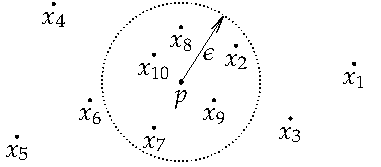
\includegraphics{figures/sequence-convergence-metric}
\caption{Sequence converging to $p$.  The first 10 points 
are shown and $M=7$ for this $\epsilon$.\label{fig:sequence-convergence-metric}}
\end{myfigureht}
\end{defn}

The limit is unique.  The proof is almost
identical (word for word) to the proof of the same fact for sequences of
real numbers,
\propref{prop:limisunique}.
Proofs of many results we know for sequences of real numbers can be
adapted to
the more general settings of metric spaces.  We must replace $\abs{x-y}$
with $d(x,y)$ in the proofs and apply the triangle inequality correctly.

\begin{prop} \label{prop:mslimisunique}
A convergent sequence in a metric space has a unique limit.
\end{prop}

\begin{proof}
%NOTE: should be word for word the same as 2.1.6
Suppose $\{ x_n \}_{n=1}^\infty$ has limits $x$ and $y$.
Take an arbitrary $\epsilon > 0$.
From the definition find an $M_1$ such that for all $n \geq M_1$,
$d(x_n,x) < \nicefrac{\epsilon}{2}$.  Similarly find an $M_2$
such that for all $n \geq M_2$, we have
$d(x_n,y) < \nicefrac{\epsilon}{2}$.  Now take an $n$ such that
$n \geq M_1$ and also $n \geq M_2$, and estimate
\begin{equation*}
\begin{split}
d(y,x)
& \leq
d(y,x_n) + d(x_n,x) \\
& <
\frac{\epsilon}{2} + \frac{\epsilon}{2} = \epsilon .
\end{split}
\end{equation*}
As $d(y,x) < \epsilon$ for all $\epsilon > 0$, then $d(x,y) = 0$
and $y=x$.  Hence the limit (if it exists) is unique.
\end{proof}

The proofs of the following propositions are left as exercises.

\begin{prop} \label{prop:msconvbound}
A convergent sequence in a metric space is bounded.
\end{prop}

\begin{prop} \label{prop:msconvifa}
A sequence $\{ x_n \}_{n=1}^\infty$ in a metric space $(X,d)$ converges to $p \in X$
if and only
if there exists a sequence $\{ a_n \}_{n=1}^\infty$ of real numbers such that
\begin{equation*}
d(x_n,p) \leq a_n \quad \text{for all } n \in \N,
\qquad
\text{and}
\qquad
\lim_{n\to\infty} a_n = 0.
\end{equation*}
\end{prop}

\begin{prop} \label{prop:mssubseq}
Let $\{ x_n \}_{n=1}^\infty$ be a sequence in a metric space $(X,d)$.
\begin{enumerate}[(i)]
\item If $\{ x_n \}_{n=1}^\infty$ converges to $p \in X$, then every
subsequence $\{ x_{n_k} \}_{k=1}^\infty$
converges to $p$.
\item If for some $K \in \N$ the $K$-tail $\{ x_n \}_{n=K+1}^\infty$
converges to $p \in X$, then
 $\{ x_n \}_{n=1}^\infty$ converges to $p$.
\end{enumerate}
\end{prop}

\begin{example}
Take $C\bigl([a,b],\R\bigr)$ be the set of continuous functions with the metric being
the uniform norm.  We saw that we obtain a metric space.
If we look at the definition of convergence, we notice that it is identical
to uniform convergence.  That is, $\{ f_n \}_{n=1}^\infty$ converges uniformly if and only
if it converges in the metric space sense.
\end{example}

\begin{remark}
It is perhaps surprising that on the set of functions $f \colon [a,b] \to
\R$ (continuous or not)
there is no metric that gives pointwise convergence.  Although the proof of
this fact is beyond the scope of this book.
\end{remark}

\subsection{Convergence in euclidean space}

In the euclidean space $\R^n$, a sequence converges if and only if every
component converges:

\begin{prop} \label{prop:msconveuc}
Let $\{ x_m \}_{m=1}^\infty$ be a sequence in $\R^n$,
where $x_m = \bigl(x_{m,1},x_{m,2},\ldots,x_{m,n}\bigr) \in \R^n$.
Then $\{ x_m \}_{m=1}^\infty$ converges if and only if
$\{ x_{m,k} \}_{m=1}^\infty$ converges for every $k=1,2,\ldots,n$, in which case
\begin{equation*}
\lim_{m\to\infty}
x_m =
\Bigl(
\lim_{m\to\infty} x_{m,1},
\lim_{m\to\infty} x_{m,2},
\ldots,
\lim_{m\to\infty} x_{m,n}
\Bigr) .
\end{equation*}
\end{prop}

\begin{proof}
Suppose
$\{ x_m \}_{m=1}^\infty$ converges to
$y = (y_1,y_2,\ldots,y_n) \in \R^n$.
Given $\epsilon > 0$, there exists an $M$ such that for all
$m \geq M$, we have
\begin{equation*}
d(y,x_m) < \epsilon.
\end{equation*}
Fix some $k=1,2,\ldots,n$.  For all $m \geq M$,
\begin{equation*}
\bigl\lvert y_k - x_{m,k} \bigr\rvert
=
\sqrt{{\bigl(y_k - x_{m,k} \bigr)}^2}
\leq
\sqrt{\sum_{\ell=1}^n {\bigl(y_\ell-x_{m,\ell}\bigr)}^2}
= d(y,x_m) < \epsilon .
\end{equation*}
Hence the sequence $\{ x_{m,k} \}_{m=1}^\infty$ converges to $y_k$.

For the other direction, suppose 
$\{ x_{m,k} \}_{m=1}^\infty$ converges to $y_k$ for every $k=1,2,\ldots,n$.
Given $\epsilon > 0$, pick an $M$ such that if $m \geq M$, then 
$\bigl\lvert y_k-x_{m,k} \bigr\rvert < \nicefrac{\epsilon}{\sqrt{n}}$ for all
$k=1,2,\ldots,n$.  Then
\begin{equation*}
d(y,x_m)
=
\sqrt{\sum_{k=1}^n {\bigl(y_k-x_{m,k}\bigr)}^2}
<
\sqrt{\sum_{k=1}^n {\left(\frac{\epsilon}{\sqrt{n}}\right)}^2}
=
\sqrt{\sum_{k=1}^n \frac{{\epsilon^2}}{n}}
= \epsilon .
\end{equation*}
That is, the sequence $\{ x_m \}_{m=1}^\infty$ converges to
$y = (y_1,y_2,\ldots,y_n) \in \R^n$.
\end{proof}

\begin{example}
As we said, the set $\C$ of complex numbers $z = x+iy$ is considered 
as the metric space $\R^2$.  The proposition says that the
sequence $\{ z_n \}_{n=1}^\infty = \{ x_n + iy_n \}_{n=1}^\infty$ converges
to $z = x+iy$
if and only if $\{ x_n \}_{n=1}^\infty$ converges to $x$ and 
$\{ y_n \}_{n=1}^\infty$ converges to $y$.
\end{example}

\subsection{Convergence and topology}

The topology---the set of open sets of a space---encodes which
sequences converge.

\begin{prop} \label{prop:msconvtopo}
Let $(X,d)$ be a metric space and $\{x_n\}_{n=1}^\infty$ a sequence in $X$.  Then
$\{ x_n \}_{n=1}^\infty$ converges to $p \in X$ if and only if for every open neighborhood
$U$ of $p$, there exists an $M \in \N$ such that for all $n \geq M$,
we have $x_n \in U$.
\end{prop}

\begin{proof}
Suppose $\{ x_n \}_{n=1}^\infty$ converges to $p$.  Let $U$ be an open neighborhood
of $p$, then there exists an $\epsilon > 0$ such that $B(p,\epsilon) \subset
U$.  As the sequence converges, find an $M \in \N$ such that for all $n \geq
M$, we have $d(p,x_n) < \epsilon$, or in other words $x_n \in B(p,\epsilon)
\subset U$.

Let us prove the other direction.  Given $\epsilon > 0$, let $U \coloneqq
B(p,\epsilon)$ be the neighborhood of $p$.  Then there is an $M \in \N$
such that for $n \geq M$, we have $x_n \in U = B(p,\epsilon)$, or in other
words, $d(p,x_n) < \epsilon$.
\end{proof}

A closed set contains the limits of its convergent sequences.

\begin{prop} \label{prop:msclosedlim}
Let $(X,d)$ be a metric space, $E \subset X$ a closed set,
and $\{ x_n \}_{n=1}^\infty$ a sequence in $E$ that converges to some $p \in X$.
Then $p \in E$.
\end{prop}

\begin{proof}
Let us prove the contrapositive.
Suppose $\{ x_n \}_{n=1}^\infty$ is a sequence in $X$ that converges to $p \in E^c$.
As $E^c$ is open, \propref{prop:msconvtopo} says that there is
an $M$ such that for all $n \geq M$,
$x_n \in E^c$.  So $\{ x_n \}_{n=1}^\infty$  is not a sequence in $E$.
\end{proof}

To take a closure of a set $A$, we start with $A$, and we throw in 
points that are limits of sequences in $A$.

\begin{prop} \label{prop:msclosureapprseq}
Let $(X,d)$ be a metric space and $A \subset X$.
Then $p \in \widebar{A}$ if and only if there exists a sequence
$\{ x_n \}_{n=1}^\infty$ of
elements in $A$ such that $\lim\limits_{n\to\infty} x_n = p$.
\end{prop}

\begin{proof}
Let $p \in \widebar{A}$.  For every $n \in \N$,
\propref{prop:msclosureappr} guarantees
a point $x_n \in B(p,\nicefrac{1}{n}) \cap A$.
As $d(p,x_n) < \nicefrac{1}{n}$, we have $\lim_{n\to\infty} x_n = p$.

For the other direction, see \exerciseref{exercise:reverseclosedseq}.
\end{proof}

\subsection{Exercises}

\begin{exercise} \label{exercise:reverseclosedseq}
Finish the proof of 
\propref{prop:msclosureapprseq}:
Let $(X,d)$ be a metric space and
$A \subset X$.  Let $p \in X$ be
such that there exists a sequence $\{ x_n \}_{n=1}^\infty$ in $A$ that converges to $p$.
Prove that $p \in \widebar{A}$.
\end{exercise}

\begin{exercise}
\leavevmode
\begin{enumerate}[a)]
\item
Show that $d(x,y) \coloneqq \min \bigl\{ 1, \abs{x-y} \bigr\}$ defines a metric on $\R$.
\item
Show that a sequence converges in $(\R,d)$ if and only if it converges
in the standard metric.
\item
Find a bounded sequence in $(\R,d)$ that
contains no convergent subsequence.
\end{enumerate}
\end{exercise}

\begin{exercise}
Prove \propref{prop:msconvbound}.
\end{exercise}

\begin{exercise}
Prove \propref{prop:msconvifa}.
\end{exercise}

\begin{exercise}
Suppose $\{x_n\}_{n=1}^\infty$ converges to $p$.  Suppose $f \colon \N
\to \N$ is a one-to-one function.  Show that
$\{ x_{f(n)} \}_{n=1}^\infty$ converges to $p$.
\end{exercise}

\begin{exercise}
Let $(X,d)$ be a metric space where $d$ is the discrete metric.  Suppose 
$\{ x_n \}_{n=1}^\infty$ is a convergent sequence in $X$.  Show that there exists
a $K \in \N$ such that for all $n \geq K$, we have $x_n = x_K$.
\end{exercise}

\begin{exercise}
A set $S \subset X$ is said to be \emph{\myindex{dense}} in $X$ if
$X \subset \widebar{S}$ or in other words if for every $p \in X$,
there exists a sequence $\{ x_n \}_{n=1}^\infty$ in $S$ that converges to $p$.
Prove that $\R^n$ contains a countable dense subset.
\end{exercise}

\begin{exercise}[Tricky]
Suppose $\{ U_n \}_{n=1}^\infty$ is a decreasing ($U_{n+1} \subset U_n$ for
all $n$) sequence of open sets in a metric space $(X,d)$ such that
$\bigcap_{n=1}^\infty U_n = \{ p \}$ for some $p \in X$.  Suppose 
$\{ x_n \}_{n=1}^\infty$ is a sequence of points in $X$ such that $x_n \in U_n$.  Does
$\{ x_n \}_{n=1}^\infty$ necessarily converge to $p$?  Prove or construct a counterexample.
\end{exercise}

\begin{exercise}
Let $E \subset X$ be closed and
let $\{ x_n \}_{n=1}^\infty$ be a sequence in $X$ converging to $p \in X$.  Suppose
$x_n \in E$ for infinitely many $n \in \N$.  Show $p \in E$.
\end{exercise}

\begin{exercise} \label{exercise:extendedrealsmetric}
Take $\R^* = \{ -\infty \} \cup \R \cup \{ \infty \}$ be the extended reals.
Define $d(x,y) \coloneqq \bigl\lvert \frac{x}{1+\abs{x}} - \frac{y}{1+\abs{y}}
\bigr\rvert$
if $x, y \in \R$,
define $d(\infty,x) \coloneqq \bigl\lvert 1 - \frac{x}{1+\abs{x}} \bigr\rvert$,
$d(-\infty,x) \coloneqq \bigl\lvert 1 + \frac{x}{1+\abs{x}} \bigr\rvert$
for all $x \in \R$, and
let $d(\infty,-\infty) \coloneqq 2$.
\begin{enumerate}[a)]
\item
Show that $(\R^*,d)$ is a metric space.
\item
Suppose $\{ x_n \}_{n=1}^\infty$ is a sequence of real numbers such that
for every $M \in \R$, there exists an $N$ such that
$x_n \geq M$ for all $n \geq N$.  Show that $\lim\limits_{n\to\infty} x_n = \infty$ in
$(\R^*,d)$.
\item
Show that a sequence of real numbers converges to a real number
in $(\R^*,d)$ if and
only if it converges in $\R$ with the standard metric.
\end{enumerate}
\end{exercise}

\begin{exercise}
Suppose $\{ V_n \}_{n=1}^\infty$ is a sequence of open sets
in $(X,d)$
such that $V_{n+1} \supset V_n$ for all $n$.  Let $\{ x_n \}_{n=1}^\infty$ be a sequence
such that $x_n \in V_{n+1} \setminus V_n$ and suppose 
$\{ x_n \}_{n=1}^\infty$ converges to $p \in X$.  Show that $p \in \partial V$
where $V = \bigcup_{n=1}^\infty V_n$.
\end{exercise}

\begin{exercise}
Prove \propref{prop:mssubseq}.
\end{exercise}

\begin{exercise}
Let $(X,d)$ be a metric space and $\{ x_n \}_{n=1}^\infty$ a sequence in $X$.
Prove that $\{ x_n \}_{n=1}^\infty$ converges to $p \in X$
if and only if
every subsequence of $\{ x_n \}_{n=1}^\infty$ has a subsequence that
converges to $p$.
\end{exercise}

\begin{exercise}
Consider $\R^n$, and let $d$ be the standard euclidean metric.
Let $d'(x,y) \coloneqq \sum_{\ell=1}^n \abs{x_\ell-y_\ell}$ and
$d''(x,y) \coloneqq \max \{ \abs{x_1-y_1},\abs{x_2-y_2},\cdots,\abs{x_n-y_n} \}$.
\begin{enumerate}[a)]
\item
Use \exerciseref{exercise:mscross}, to show that
$(\R^n,d')$ and
$(\R^n,d'')$ are metric spaces.
\item
Let $\{ x_k \}_{k=1}^\infty$ be a sequence in $\R^n$ and $p \in \R^n$.
Prove that the following statements are equivalent:
\begin{enumerate}[(1)]
\item
$\{ x_k \}_{k=1}^\infty$ converges to $p$ in $(\R^n,d)$.
\item
$\{ x_k \}_{k=1}^\infty$ converges to $p$ in $(\R^n,d')$.
\item
$\{ x_k \}_{k=1}^\infty$ converges to $p$ in $(\R^n,d'')$.
\end{enumerate}
\end{enumerate}
\end{exercise}

%%%%%%%%%%%%%%%%%%%%%%%%%%%%%%%%%%%%%%%%%%%%%%%%%%%%%%%%%%%%%%%%%%%%%%%%%%%%%%

\sectionnewpage
\section{Completeness and compactness}
\label{sec:metcompact}

%mbxINTROSUBSECTION

\sectionnotes{2 lectures}

\subsection{Cauchy sequences and completeness}

Just like with sequences of real numbers, we define Cauchy sequences.

\begin{defn}
Let $(X,d)$ be a metric space.
A sequence $\{ x_n \}_{n=1}^\infty$ in $X$ is a \emph{\myindex{Cauchy sequence}} if
for every $\epsilon > 0$, there exists an $M \in \N$ such that
for all $n \geq M$ and all $k \geq M$, we have
\begin{equation*}
d(x_n, x_k) < \epsilon .
\end{equation*}
\end{defn}

The definition is again simply a translation of the concept
from the real numbers to metric spaces.  A sequence of real
numbers is Cauchy in the sense of \chapterref{seq:chapter} if and only if
it is Cauchy in the sense above, provided we equip the real numbers with
the standard metric $d(x,y) = \abs{x-y}$.

\begin{prop}
A convergent sequence in a metric space is Cauchy.
\end{prop}

\begin{proof}
Suppose $\{ x_n \}_{n=1}^\infty$ converges to $p$.
Given $\epsilon > 0$, there is an $M$ such that for all $n \geq M$,
we have $d(p,x_n) < \nicefrac{\epsilon}{2}$.  Hence
for all $n,k \geq M$, we have
$d(x_n,x_k) \leq d(x_n,x) + d(x,x_k) < \nicefrac{\epsilon}{2} +
\nicefrac{\epsilon}{2} = \epsilon$.
\end{proof}

\begin{defn}
We say a metric space $(X,d)$ is
\emph{\myindex{complete}} or \emph{\myindex{Cauchy-complete}}
if every Cauchy sequence $\{ x_n \}_{n=1}^\infty$ in $X$
converges to a $p \in X$.
\end{defn}

\begin{prop}
The space $\R^n$ with the standard metric is a complete metric space.
\end{prop}

For $\R = \R^1$, completeness was proved in \chapterref{seq:chapter}.
The proof of completeness in $\R^n$
is a reduction to the one-dimensional case.

\begin{proof}
Let $\{ x_m \}_{m=1}^\infty$ be a Cauchy sequence
in $\R^n$, where $x_m = \bigl(x_{m,1},x_{m,2},\ldots,x_{m,n}\bigr) \in \R^n$.
As the sequence is Cauchy, given $\epsilon > 0$, there exists an $M$ such that for all
$i,j \geq M$,
\begin{equation*}
d(x_i,x_j) < \epsilon.
\end{equation*}

Fix some $k=1,2,\ldots,n$.  For $i,j \geq M$,
\begin{equation*}
\bigl\lvert x_{i,k} - x_{j,k} \bigr\rvert
=
\sqrt{{\bigl(x_{i,k} - x_{j,k}\bigr)}^2}
\leq
\sqrt{\sum_{\ell=1}^n {\bigl(x_{i,\ell}-x_{j,\ell}\bigr)}^2}
= d(x_i,x_j) < \epsilon .
\end{equation*}
Hence the sequence $\{ x_{m,k} \}_{m=1}^\infty$ is Cauchy.  As $\R$ is
complete the sequence converges; there exists a $y_k \in \R$ such that
$y_k = \lim_{m\to\infty} x_{m,k}$.
Write $y = (y_1,y_2,\ldots,y_n) \in \R^n$.
By \propref{prop:msconveuc}, $\{ x_m \}_{m=1}^\infty$ converges
to $y \in \R^n$, and hence $\R^n$ is complete.
\end{proof}

In the language of metric spaces,
the results on continuity of section \sectionref{sec:liminter},
say that the metric space
$C\bigl([a,b],\R\bigr)$ of \exampleref{example:msC01} is complete.
The proof follows by \myquote{unrolling the definitions,} 
and is left as \exerciseref{exercise:CabRcomplete}.

\begin{prop} \label{prop:CabRcomplete}
The space of continuous functions $C\bigl([a,b],\R\bigr)$ with the uniform
norm as metric is a complete metric space.
\end{prop}

A subset of a complete metric space such as $\R^n$ with the subspace metric need not be
complete.  For example, $(0,1]$ with the subspace metric is not
complete, as $\{ \nicefrac{1}{n} \}_{n=1}^\infty$ is a Cauchy sequence in $(0,1]$
with no limit in $(0,1]$.
However, 
a closed subspace of a complete metric space is
complete.  After all, one way
to think of a closed set is that it contains all points
reachable from the set via a sequence.
The proof is 
\exerciseref{exercise:closedcomplete}.

\begin{prop} \label{prop:closedcomplete}
Suppose $(X,d)$ is a complete metric space and $E \subset X$
is closed.
Then $E$ is a complete metric space with the subspace metric.
\end{prop}

\subsection{Compactness}

\begin{defn}
Let $(X,d)$ be a metric space and $K \subset X$. 
The set $K$ is said to be \emph{\myindex{compact}}
if for every collection
of open sets $\{ U_{\lambda} \}_{\lambda \in I}$ such that
\begin{equation*}
K \subset \bigcup_{\lambda \in I} U_\lambda ,
\end{equation*}
there exists a finite subset
$\{ \lambda_1, \lambda_2,\ldots,\lambda_m \} \subset I$
such that
\begin{equation*}
K \subset \bigcup_{j=1}^m U_{\lambda_j} .
\end{equation*}
\end{defn}

A collection of open sets $\{ U_{\lambda} \}_{\lambda \in I}$ as above is
said to be an \emph{\myindex{open cover}} of $K$.  A way to say that
$K$ is compact is to say that \emph{every open cover of $K$ has a finite
\myindex{subcover}}.

\begin{example}
Let $\R$ be the metric space with the standard metric.

The set $\R$ is not compact.  Proof: For $j \in \N$, let $U_j \coloneqq (-j,j)$.
Any $x \in \R$ is in some $U_j$ (by the
\hyperref[thm:arch:i]{Archimedean property}), so we have an open cover.
Suppose we have a finite
subcover $\R \subset U_{j_1} \cup U_{j_2} \cup \cdots \cup U_{j_m}$,
and suppose $j_1 < j_2 < \cdots < j_m$.  Then $\R \subset U_{j_m}$, but that is
a contradiction as $j_m \in \R$ on one hand and $j_m \notin U_{j_m} =
(-j_m,j_m)$ on the
other.

The set $(0,1) \subset \R$ is also not compact.  Proof:  Take the 
sets $U_{j} \coloneqq (\nicefrac{1}{j},1-\nicefrac{1}{j})$ for $j=3,4,5,\ldots$.
As above $(0,1) = \bigcup_{j=3}^\infty U_j$.  And similarly as above,
if there exists a finite subcover, then there is one $U_j$ such that $(0,1)
\subset U_j$, which again leads to a contradiction.

The set $\{ 0 \} \subset \R$ is compact.  Proof: Given an open cover $\{
U_{\lambda} \}_{\lambda \in I}$, there must exist a $\lambda_0$ such that $0
\in U_{\lambda_0}$ as it is a cover.  But then $U_{\lambda_0}$ gives a
finite subcover.

We will prove below that $[0,1]$, and in fact every closed and bounded
interval $[a,b]$, is compact.
\end{example}

\begin{prop}
Let $(X,d)$ be a metric space.  If $K \subset X$ is compact, then
$K$ is closed and bounded.
\end{prop}

\begin{proof}
First, we prove that a compact set is bounded.
Fix $p \in X$.  We have the open cover
\begin{equation*}
K \subset \bigcup_{n=1}^\infty B(p,n) = X .
\end{equation*}
If $K$ is compact, then there exists some set of indices
$n_1 < n_2 < \ldots < n_m$ such that
\begin{equation*}
K \subset \bigcup_{j=1}^m B(p,n_j) = B(p,n_m) .
\end{equation*}
As $K$ is contained in a ball, $K$ is bounded.
See the left-hand side of \figureref{fig:compactbndclosed}.

Next, we show a set that is not closed is not compact.  Suppose 
$\widebar{K} \not= K$, that is, there is a point $x \in \widebar{K}
\setminus K$.
If $y \not= x$, then
$y \notin C(x,\nicefrac{1}{n})$
for $n \in \N$
such that $\nicefrac{1}{n} < d(x,y)$.
Furthermore, $x \notin K$, so
\begin{equation*}
K \subset \bigcup_{n=1}^\infty {C(x,\nicefrac{1}{n})}^c .
\end{equation*}
A closed ball is closed, so its complement ${C(x,\nicefrac{1}{n})}^c$ is open, and
we have an open cover.
If we take any
finite collection of indices $n_1 < n_2 < \ldots < n_m$, then 
\begin{equation*}
\bigcup_{j=1}^m {C(x,\nicefrac{1}{n_j})}^c 
=
{C(x,\nicefrac{1}{n_m})}^c 
\end{equation*}
As $x$ is in the closure of $K$,
then
$C(x,\nicefrac{1}{n_m}) \cap K \not= \emptyset$.  So there is no
finite subcover and $K$ is not compact.
See the right-hand side of \figureref{fig:compactbndclosed}.
\end{proof}

\begin{myfigureht}
\subimport*{figures/}{compact_bnd_closed.pdf_t}
\caption{Proving compact set is bounded (left) and closed (right).\label{fig:compactbndclosed}}
\end{myfigureht}

We prove below that 
in a finite-dimensional euclidean space,
every closed bounded set is compact.
So closed bounded sets
of $\R^n$ are examples of compact sets.
It is not true that in every metric space, closed and bounded is equivalent
to compact.  A simple example is an incomplete metric space such as
$(0,1)$ with the subspace metric from $\R$.
There are many complete and very useful metric spaces
where closed and bounded is not
enough to give compactness: $C\bigl([a,b],\R\bigr)$ is a complete metric
space, but the closed unit ball $C(0,1)$ is not compact, see
\exerciseref{exercise:msclbounnotcompt}.  However, see also
\exerciseref{exercise:mstotbound}.

Not worrying about the boundedness for a moment,
note further the difference between being closed and being compact.  Being
closed depends on the ambient metric space:
The set $(0,1]$ is not closed in $\R$,
but it is closed in the subspace $(0,\infty)$.
However, a set $K$ is compact
in some metric space $(X,d)$ if and only if it is compact in the subspace
metric on $K$.  So for a compact set, we do not have to ask
what metric space it lives in.
On the other hand, every set is always closed in the 
subspace metric as a subset of itself.
See also \exerciseref{exercise:subspacecompact}.

A useful property of compact sets in a metric space is that every
sequence in the set has a convergent subsequence converging
to a point in the set.
Such sets are called
\emph{\myindex{sequentially compact}}.
We will prove that in the
context of metric spaces, a set is compact if and only if it is sequentially
compact.
First we prove a lemma.

\begin{lemma}[Lebesgue covering lemma%
\footnote{Named after the French mathematician
\href{https://en.wikipedia.org/wiki/Henri_Lebesgue}{Henri L\'eon Lebesgue}
(1875--1941).
The number $\delta$ is sometimes called the \myindex{Lebesgue number} of the
cover.}]\label{ms:lebesgue}
\index{Lebesgue covering lemma}
Let $(X,d)$ be a metric space and $K \subset X$.  Suppose 
every sequence in $K$ has a subsequence convergent in $K$.  Given
an open cover $\{ U_\lambda \}_{\lambda \in I}$ of $K$, there exists a
$\delta > 0$ such that for every $x \in K$, there exists a $\lambda \in I$
with $B(x,\delta) \subset U_\lambda$.
\end{lemma}

\begin{proof}
We prove the lemma by contrapositive.
If the conclusion is not true, then
there is
an open cover $\{ U_\lambda \}_{\lambda \in I}$ of $K$ with
the following property.
For every $n \in \N$, there exists an $x_n \in K$ such that
$B(x_n,\nicefrac{1}{n})$ is not a subset of any $U_\lambda$.
Take any $x \in K$.  There is
a $\lambda \in I$ such that $x \in U_\lambda$.  As $U_\lambda$ is open,
there is an $\epsilon > 0$ 
such that $B(x,\epsilon) \subset U_\lambda$.  Take $M$ such that
$\nicefrac{1}{M} < \nicefrac{\epsilon}{2}$.  If $y \in 
B(x,\nicefrac{\epsilon}{2})$ and $n \geq M$, then 
\begin{equation*}
B(y,\nicefrac{1}{n}) \subset
B(y,\nicefrac{1}{M}) \subset
B(y,\nicefrac{\epsilon}{2}) \subset B(x,\epsilon)
\subset U_\lambda ,
\end{equation*}
where 
$B(y,\nicefrac{\epsilon}{2}) \subset B(x,\epsilon)$
follows by triangle inequality.
See \figureref{fig:lebesguedelta}.
Thus $y \not= x_n$.
In other words, for all $n \geq M$, $x_n \notin B(x,\nicefrac{\epsilon}{2})$. 
The sequence cannot have a subsequence converging to $x$.  As $x \in K$ was
arbitrary we are done.
\end{proof}

\begin{myfigureht}
\subimport*{figures/}{lebesguedelta.pdf_t}
\caption{Proof of Lebesgue covering lemma.
Note that $B(y,\nicefrac{\epsilon}{2}) \subset
B(x,\epsilon)$ by triangle inequality.\label{fig:lebesguedelta}}
\end{myfigureht}

It is important to recognize what the lemma says.  It says that
if $K$ is sequentially compact, then given any
cover there is a single $\delta > 0$.  The $\delta$ depends on the cover,
but, of course, it does not depend on $x$.

For example, let $K \coloneqq [-10,10]$ and let
$U_n \coloneqq (n,n+2)$ for $n \in \Z$
give an open cover.
Consider $x \in K$. There is an $n \in \Z$, 
such that $n \leq x < n+1$.
If $n \leq x < n+\nicefrac{1}{2}$, then
$B\bigl(x,\nicefrac{1}{2}\bigr) \subset U_{n-1}$.
If $n+ \nicefrac{1}{2} \leq x < n+1$, then
$B\bigl(x,\nicefrac{1}{2}\bigr) \subset U_{n}$.  So $\delta =
\nicefrac{1}{2}$ will do.  The sets 
$U'_n \coloneqq \bigl(\frac{n}{2},\frac{n+2}{2} \bigr)$,
again give an open cover,
but now the largest $\delta$ that works is $\nicefrac{1}{4}$.

On the other hand, $\N \subset \R$ is not sequentially compact.
It is an exercise to find a cover for which no $\delta > 0$ works.


\begin{thm} \label{thm:mscompactisseqcpt}
Let $(X,d)$ be a metric space.  Then $K \subset X$ is compact if
and only if every sequence in $K$ has a subsequence converging to
a point in $K$.
\end{thm}

\begin{proof}
Claim: \emph{Let $K \subset X$ be a subset of $X$ and
$\{ x_n \}_{n=1}^\infty$ a sequence in $K$.  Suppose that for each $x \in K$,
there is a ball $B(x,\alpha_x)$ for some $\alpha_x > 0$ such that
$x_n \in B(x,\alpha_x)$ for only finitely many $n \in \N$.
Then $K$ is not compact.}

Proof of the claim:
Notice
\begin{equation*}
K \subset \bigcup_{x \in K} B(x,\alpha_x) .
\end{equation*}
Any finite collection of these balls contains at most finitely many
elements of $\{ x_n \}_{n=1}^\infty$,
and so there must be an $x_n \in K$
not in their union.  Hence, $K$ is not compact and the claim is
proved.

So suppose that $K$ is compact and $\{ x_n \}_{n=1}^\infty$ is a sequence in $K$.
Then there exists an $x \in K$ such that
for all $\delta > 0$,
$B(x,\delta)$ contains $x_n$ for infinitely many $n \in \N$.
We define the subsequence inductively.
The ball $B(x,1)$ contains some $x_k$, so let $n_1 \coloneqq k$.
Suppose $n_{j-1}$ is defined.
There must exist a $k > n_{j-1}$
such that $x_k \in B(x,\nicefrac{1}{j})$.  Define
$n_j \coloneqq k$.
We now posses a subsequence $\{ x_{n_j} \}_{j=1}^\infty$.
Since
$d(x,x_{n_j}) < \nicefrac{1}{j}$,  \propref{prop:msconvifa} says
$\lim_{j\to\infty} x_{n_j} = x$.

For the other direction, suppose every sequence in~$K$
has a 
subsequence converging in~$K$.
Take
an open cover $\{ U_\lambda \}_{\lambda \in I}$ of $K$.
Using the Lebesgue covering lemma above, find a $\delta > 0$
such that for every $x \in K$, there is a $\lambda \in I$ with
$B(x,\delta) \subset U_\lambda$.

Pick $x_1 \in K$ and find $\lambda_1 \in I$ such that $B(x_1,\delta) \subset
U_{\lambda_1}$.
If $K \subset U_{\lambda_1}$, we stop as we have found a
finite subcover.
Otherwise, there must be
a point $x_2 \in K \setminus U_{\lambda_1}$.
Note that $d(x_2,x_1) \geq \delta$.
There must exist some $\lambda_2 \in I$ such that
$B(x_2,\delta) \subset U_{\lambda_2}$.
We work inductively.  Suppose $\lambda_{n-1}$ is defined.
Either
$U_{\lambda_1} \cup
U_{\lambda_2} \cup \cdots \cup
U_{\lambda_{n-1}}$ is a finite cover of $K$, in which case we
stop, or
there must be 
a point $x_n \in K \setminus \bigl( U_{\lambda_1} \cup
U_{\lambda_2} \cup \cdots \cup
U_{\lambda_{n-1}}\bigr)$.
Note that $d(x_n,x_j) \geq \delta$ for all $j = 1,2,\ldots,n-1$.
Next, there must be some $\lambda_n \in I$
such that $B(x_n,\delta) \subset U_{\lambda_n}$.
See \figureref{fig:seqcompactiscompact}.

\begin{myfigureht}
\subimport*{figures/}{seqcompactiscompact.pdf_t}
\caption{Covering $K$ by $U_{\lambda}$.  The points
$x_1,x_2,x_3,x_4$, 
the three sets 
$U_{\lambda_1}$,
$U_{\lambda_2}$,
$U_{\lambda_2}$,
and 
the first three balls
of radius $\delta$ are drawn.\label{fig:seqcompactiscompact}}
\end{myfigureht}

Either at some point we obtain a finite subcover of $K$,
or we obtain an
infinite
sequence $\{ x_n \}_{n=1}^\infty$ as above.
For contradiction, suppose that
there is no finite subcover and we have the sequence $\{ x_n \}_{n=1}^\infty$.
For all $n$ and $k$, $n \not= k$, 
we have $d(x_n,x_k) \geq \delta$.
So no subsequence of $\{ x_n \}_{n=1}^\infty$ is Cauchy.
Hence, no subsequence of $\{ x_n \}_{n=1}^\infty$ is convergent,
which is a contradiction.
\end{proof}

\begin{example} \label{example:intervalcompact}
\thmref{thm:bwseq},
the Bolzano--Weierstrass theorem for sequences of real numbers,
says that every bounded sequence in $\R$ has a convergent
subsequence.  Therefore, every sequence in a closed interval $[a,b] \subset \R$ has 
a convergent subsequence.  The limit is also in $[a,b]$ as limits
preserve non-strict inequalities.  Hence a closed bounded interval $[a,b]
\subset \R$ is (sequentially) compact.
\end{example}

\begin{prop} \label{prop:closedsubsetcompact}
Let $(X,d)$ be a metric space and let $K \subset X$ be compact.  If
$E \subset K$ is a closed set, then $E$ is compact.
\end{prop}

Because $K$ is closed, $E$ is closed in $K$ if
and only if it is closed in $X$.
See \propref{prop:topology:subspacesame}.

\begin{proof}
Let $\{ x_n \}_{n=1}^\infty$ be a sequence in $E$.  It is also a sequence in $K$.
Therefore, it has a convergent subsequence $\{ x_{n_j} \}_{j=1}^\infty$ that converges to
some $x \in K$.  As $E$ is closed the limit of a sequence in $E$ is also in $E$
and so $x \in E$.  Thus $E$ must be compact.
\end{proof}

\begin{thm}[Heine--Borel%
\footnote{Named after the German mathematician 
\href{https://en.wikipedia.org/wiki/Eduard_Heine}{Heinrich Eduard Heine}
(1821--1881),
and the French mathematician
\href{https://en.wikipedia.org/wiki/\%C3\%89mile_Borel}{F\'elix \'Edouard Justin \'Emile Borel}
(1871--1956).}]%
\index{Heine--Borel theorem}
\label{thm:msbw}
A closed bounded subset $K \subset \R^n$ is compact.
\end{thm}

So subsets of $\R^n$ are compact if and only if they are closed and bounded,
a condition that is much easier to check.
Let us reiterate that the Heine--Borel theorem only holds for $\R^n$ and not
for metric spaces in general.
The theorem does not hold even for subspaces of $\R^n$, just in $\R^n$
itself.
In general, compact implies closed and
bounded, but not vice versa.

\begin{proof}
For $\R = \R^1$, suppose $K \subset \R$ is closed and bounded.
Then $K \subset [a,b]$ for some closed and bounded interval,
which is compact by \exampleref{example:intervalcompact}.
As $K$ is a closed subset of a compact set,
it is compact by \propref{prop:closedsubsetcompact}.

We carry out the proof for $n=2$ and leave arbitrary $n$ as an exercise.
As $K \subset \R^2$ is bounded, there exists a set
$B=[a,b]\times[c,d] \subset \R^2$ such that $K \subset B$.  We will show
that $B$ is compact.  Then $K$, being a closed subset of a compact $B$, is
also compact.  

Let $\bigl\{ (x_k,y_k) \bigr\}_{k=1}^\infty$ be a sequence in $B$.  That is,
$a \leq x_k \leq b$ and
$c \leq y_k \leq d$ for all $k$.  A bounded sequence of real numbers
has a convergent
subsequence so there is a subsequence $\{ x_{k_j} \}_{j=1}^\infty$
that is convergent.  The subsequence 
$\{ y_{k_j} \}_{j=1}^\infty$ is also a bounded sequence so there exists
a subsequence
$\{ y_{k_{j_i}} \}_{i=1}^\infty$ that is convergent.  A subsequence of a
convergent sequence is still convergent, so 
$\{ x_{k_{j_i}} \}_{i=1}^\infty$ is convergent.
Let
\begin{equation*}
x \coloneqq \lim_{i\to\infty} x_{k_{j_i}}
\qquad \text{and} \qquad
y \coloneqq \lim_{i\to\infty} y_{k_{j_i}} .
\end{equation*}
By \propref{prop:msconveuc},
$\bigl\{ (x_{k_{j_i}},y_{k_{j_i}}) \bigr\}_{i=1}^\infty$ converges to $(x,y)$.
Furthermore, as $a \leq x_k \leq b$ and
$c \leq y_k \leq d$ for all $k$, we know that $(x,y) \in B$.
\end{proof}

\begin{example}
The discrete metric provides interesting counterexamples again.
Let $(X,d)$ be a metric space with the discrete metric, that is, $d(x,y) = 1$
if $x \not= y$.  Suppose
$X$ is an infinite set.  Then
\begin{enumerate}[(i)]
\item $(X,d)$ is a complete metric space.
\item Any subset $K \subset X$ is closed and bounded.
\item A subset $K \subset X$ is compact if and only if it is a finite set.
\item The conclusion of the Lebesgue covering lemma is always satisfied,
e.g. with $\delta = \nicefrac{1}{2}$,
even for noncompact $K \subset X$.
\end{enumerate}
The proofs
of the statements above are either trivial or are relegated to the exercises
below.
\end{example}

\begin{remark}
A subtle issue with Cauchy sequences, completeness, compactness,
and convergence is that compactness and convergence only depend on the
topology, that is, on which sets are the open sets.  On the other hand,
Cauchy sequences and completeness depend on the actual metric.
See \exerciseref{exercise:cauchydepndsonmetric}.
\end{remark}

\subsection{Exercises}

\begin{exercise}
Let $(X,d)$ be a metric space and $A$ a finite subset of $X$.
Show that $A$ is compact.
\end{exercise}

\begin{samepage}
\begin{exercise}
Let $A \coloneqq \{ \nicefrac{1}{n} : n \in \N \} \subset \R$.
\begin{enumerate}[a)]
\item
Show that $A$ is
not compact directly using the definition.
\item
Show that $A \cup \{ 0 \}$ is
compact directly using the definition.
\end{enumerate}
\end{exercise}
\end{samepage}


\begin{exercise}
Let $(X,d)$ be a metric space with the discrete metric.
\begin{enumerate}[a)]
\item
Prove that $X$ is complete.
\item
Prove that $X$ is compact if and only if $X$ is a finite set.
\end{enumerate}
\end{exercise}

\begin{exercise}
\leavevmode
\begin{enumerate}[a)]
\item
Show that the union of finitely many compact sets is a compact set.
\item
Find an example where the union of infinitely many compact sets is not
compact.
\end{enumerate}
\end{exercise}

\begin{exercise}
Prove \thmref{thm:msbw} for arbitrary dimension.
Hint: The trick is to use the correct notation.
\end{exercise}

\begin{exercise} \label{exercise:subspacecompact}
Show that a compact set $K$ (in any metric space)
is itself a complete metric space (using the subspace metric).
\end{exercise}

\begin{exercise} \label{exercise:CabRcomplete}
Let $C\bigl([a,b],\R\bigr)$ be the metric space as in \exampleref{example:msC01}.  Show that
$C\bigl([a,b],\R\bigr)$ is a complete metric space.
\end{exercise}

\begin{exercise}[Challenging] \label{exercise:msclbounnotcompt}
Let $C\bigl([0,1],\R\bigr)$ be the metric space of \exampleref{example:msC01}.  Let $0$
denote the zero function.  Then show that the closed ball
$C(0,1)$ is not compact (even though it is closed and bounded).
Hints: Construct a sequence of distinct continuous functions
$\{ f_n \}_{n=1}^\infty$ such that
$d(f_n,0) = 1$ and $d(f_n,f_k) = 1$ for all $n \not= k$.  Show that
the set $\{ f_n : n \in \N \} \subset C(0,1)$ is closed but not compact.
See \chapterref{fs:chapter} for inspiration.
\end{exercise}

\begin{exercise}[Challenging]
Show that there exists a metric on $\R$ that makes $\R$ into a compact set.
\end{exercise}

\begin{exercise}
Suppose $(X,d)$ is complete and suppose we have a countably infinite
collection of nonempty compact sets $E_1 \supset E_2 \supset E_3 \supset
\cdots$.  Prove $\bigcap_{j=1}^\infty E_j \not= \emptyset$.
\end{exercise}

\begin{exercise}[Challenging]
Let $C\bigl([0,1],\R\bigr)$ be the metric space of \exampleref{example:msC01}.
Let $K$ be the set of $f \in C\bigl([0,1],\R\bigr)$ such that
$f$ is equal to a quadratic polynomial, i.e.\ $f(x) = a+bx+cx^2$, and such that
$\abs{f(x)} \leq 1$ for all $x \in [0,1]$,
that is $f \in C(0,1)$.  Show that $K$ is compact.
\end{exercise}

\begin{exercise}[Challenging] \label{exercise:mstotbound}
Let $(X,d)$ be a complete metric space.
Show that $K \subset X$ is compact if and only if $K$ is closed
and such that for every $\epsilon > 0$
there exists a finite set of points $x_1,x_2,\ldots,x_n$ with
$K \subset \bigcup_{j=1}^n B(x_j,\epsilon)$.
Note: Such a set $K$ is said to be \emph{\myindex{totally bounded}},
so in a complete metric space a set is compact if and only
if it is closed and totally bounded.
\end{exercise}

\begin{exercise}
Take $\N \subset \R$ using the standard metric.  Find an open cover of $\N$
such that the conclusion of the Lebesgue covering lemma does not hold.
\end{exercise}

\begin{exercise}
Prove the general \myindex{Bolzano--Weierstrass theorem}:
Any bounded sequence $\{ x_k \}_{k=1}^\infty$ in $\R^n$
has a convergent subsequence.
\end{exercise}

\begin{exercise}
Let $X$ be a metric space and
$C \subset \sP(X)$ the set of nonempty compact subsets of $X$.
Using the Hausdorff metric from \exerciseref{exercise:mshausdorffpseudo},
show that $(C,d_H)$ is a metric space.  That is, show that
if $L$ and $K$ are nonempty compact subsets, then $d_H(L,K) = 0$
if and only if $L=K$.
\end{exercise}

\begin{exercise} \label{exercise:closedcomplete}
Prove \propref{prop:closedcomplete}.  That is,
let $(X,d)$ be a complete metric space and $E \subset X$ a closed set.
Show that $E$ with the subspace metric is a complete metric space.
\end{exercise}

\begin{exercise}
Let $(X,d)$ be an incomplete metric space.  Show that there exists a
closed and bounded set $E \subset X$ that is not compact.
\end{exercise}

\begin{exercise}
Let $(X,d)$ be a metric space and $K \subset X$.
Prove that $K$ is compact as a subset of $(X,d)$ if and only if $K$ is
compact as a subset of itself with the subspace metric.
\end{exercise}

\begin{exercise} \label{exercise:cauchydepndsonmetric}
Consider two metrics on $\R$.
Let $d(x,y) \coloneqq \abs{x-y}$ be the standard metric,
and let
$d'(x,y) \coloneqq \bigl\lvert \frac{x}{1+\abs{x}} - \frac{y}{1+\abs{y}}
\bigr\rvert$.
\begin{enumerate}[a)]
\item
Show that $(\R,d')$ is a metric space (if you have done
\exerciseref{exercise:extendedrealsmetric}, the computation is the same).
\item
Show that the topology is the same, that is, a set is open in
$(\R,d)$ if and only if it is open in $(\R,d')$.
\item
Show that a set is compact in
$(\R,d)$ if and only if it is compact in $(\R,d')$.
\item
Show that a sequence converges in $(\R,d)$ if and only if
it converges in $(\R,d')$.
\item
Find a sequence of real numbers that is Cauchy
in $(\R,d')$ but not Cauchy in $(\R,d)$.
\item
While $(\R,d)$ is complete, show that $(\R,d')$ is not complete.
\end{enumerate}
\end{exercise}

\begin{exercise} \label{exercise:relativelycompactseq}
\pagebreak[2]
Let $(X,d)$ be a complete metric space.
We say a set $S \subset X$ is \emph{\myindex{relatively compact}}
if the closure $\widebar{S}$ is compact.
Prove that $S \subset X$ is relatively compact if and only if
given any sequence $\{ x_n \}_{n=1}^\infty$ in $S$, there exists a subsequence
$\{ x_{n_k} \}_{k=1}^\infty$ that converges (in $X$).
\end{exercise}

%%%%%%%%%%%%%%%%%%%%%%%%%%%%%%%%%%%%%%%%%%%%%%%%%%%%%%%%%%%%%%%%%%%%%%%%%%%%%%

\sectionnewpage
\section{Continuous functions}
\label{sec:metcont}

%mbxINTROSUBSECTION

\sectionnotes{1.5--2 lectures}

\subsection{Continuity}

\begin{defn}
Let $(X,d_X)$ and $(Y,d_Y)$ be metric spaces and $c \in X$.
Then $f \colon X \to Y$ is
\emph{continuous at $c$}\index{continuous at $c$}
if for every $\epsilon > 0$
there is a $\delta > 0$ such that whenever $x \in X$ and $d_X(x,c) <
\delta$, then
$d_Y\bigl(f(x),f(c)\bigr) < \epsilon$.

\medskip

When $f \colon X \to Y$ is continuous at all $c \in X$, we simply say
that $f$ is a \emph{continuous function}\index{continuous function!in a
metric space}\index{function!continuous}.
\end{defn}

The definition agrees with the definition from \chapterref{lim:chapter} when
$f$ is a real-valued function on the real line---as long as we take the standard
metric on $\R$, of course.

\begin{prop} \label{prop:contiscont}
Let $(X,d_X)$ and $(Y,d_Y)$ be metric spaces.
Then $f \colon X \to Y$ is
continuous at $c \in X$
if and only if for every sequence $\{ x_n \}_{n=1}^\infty$ in $X$
converging to $c$, the sequence $\bigl\{ f(x_n) \bigr\}_{n=1}^\infty$ converges
to $f(c)$.
\end{prop}

\begin{proof}
Suppose $f$ is continuous at $c$.  Let $\{ x_n \}_{n=1}^\infty$ be a
sequence in $X$ converging to $c$.  Given $\epsilon > 0$,
there is a $\delta > 0$ such that $d_X(x,c) < \delta$ implies
$d_Y\bigl(f(x),f(c)\bigr) < \epsilon$.  So take $M$ such that
for all $n \geq M$, we have $d_X(x_n,c) < \delta$, then
$d_Y\bigl(f(x_n),f(c)\bigr) < \epsilon$.  Hence $\bigl\{ f(x_n) \bigr\}_{n=1}^\infty$
converges to $f(c)$.

On the other hand, suppose $f$ is not continuous at $c$.
Then there exists an $\epsilon > 0$,
such that for every $n \in \N$ there exists an $x_n \in X$,
with
$d_X(x_n,c) < \nicefrac{1}{n}$ such that $d_Y\bigl(f(x_n),f(c)\bigr) \geq
\epsilon$.  Then $\{ x_n \}_{n=1}^\infty$ converges to $c$, but
$\bigl\{ f(x_n) \bigr\}_{n=1}^\infty$
does not converge to $f(c)$.
\end{proof}

\begin{example}
Suppose $f \colon \R^2 \to \R$ is a polynomial.  That is,
\begin{equation*}
f(x,y) =
\sum_{j=0}^d
\sum_{k=0}^{d-j}
a_{jk}\,x^jy^k =
a_{0\,0} + a_{1\,0} \, x +
a_{0\,1} \, y+  
a_{2\,0} \, x^2+  
a_{1\,1} \, xy+  
a_{0\,2} \, y^2+ \cdots +
a_{0\,d} \, y^d ,
\end{equation*}
for some $d \in \N$ (the degree) and $a_{jk} \in \R$.  We claim 
$f$ is continuous.  Let $\bigl\{ (x_n,y_n) \bigr\}_{n=1}^\infty$ be a sequence
in $\R^2$ that converges to $(x,y) \in \R^2$.  We proved that this
means $\lim_{n\to\infty} x_n = x$ and $\lim_{n\to\infty} y_n = y$.
By \propref{prop:contalg},
\begin{equation*}
\lim_{n\to\infty}
f(x_n,y_n) =
\lim_{n\to\infty}
\sum_{j=0}^d
\sum_{k=0}^{d-j}
a_{jk} \, x_n^jy_n^k 
=
\sum_{j=0}^d
\sum_{k=0}^{d-j}
a_{jk} \, x^jy^k
=
f(x,y) .
\end{equation*}
So $f$ is continuous at $(x,y)$, and as $(x,y)$ was arbitrary $f$ is
continuous everywhere.  Similarly, a
polynomial in $n$ variables is continuous.
\end{example}

Be careful about taking limits separately.
Consider $f \colon \R^2 \to \R$ defined by $f(x,y) \coloneqq \frac{xy}{x^2+y^2}$
outside the origin and $f(0,0) \coloneqq 0$.
See \figureref{fig:xyxsqysq}.
In \exerciseref{exercise:dicontR2},
you are asked to prove that $f$ is not continuous at the origin.
However, for every $y$, the function $g(x) \coloneqq f(x,y)$ is
continuous,
and for every $x$, the function $h(y) \coloneqq f(x,y)$ is continuous.
\begin{myfigureht}
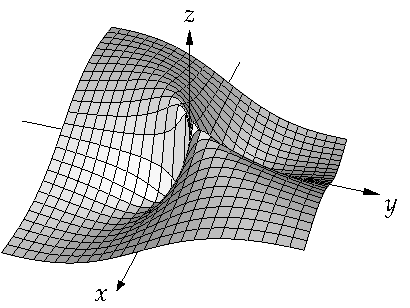
\includegraphics{figures/xyxsqysq}
\caption{Graph of $\frac{xy}{x^2+y^2}$.\label{fig:xyxsqysq}}
\end{myfigureht}

\begin{example}
Let $X$ be a metric space and $f \colon X \to \C$ a complex-valued
function.  Write $f(p) = g(p) + i \, h(p)$, where $g \colon X \to \R$
and $h \colon X \to \R$ are the real and imaginary parts of $f$.
Then $f$ is continuous at $c \in X$ if and only if its real
and imaginary parts are continuous at~$c$.  
This fact follows because $\bigl\{ f(p_n) = g(p_n) + i \, h(p_n) \bigr\}_{n=1}^\infty$
converges to $f(p) = g(p) + i \, h(p)$ if and only if
$\bigl\{ g(p_n) \bigr\}_{n=1}^\infty$ converges to $g(p)$ and
$\bigl\{ h(p_n) \bigr\}_{n=1}^\infty$ converges to $h(p)$.
\end{example}

\subsection{Compactness and continuity}

Continuous maps do not map closed sets to closed sets.  For example,
$f \colon (0,1) \to \R$ defined by $f(x) \coloneqq x$ takes the set $(0,1)$, which
is closed in $(0,1)$, to the set $(0,1)$, which is not closed in $\R$.
On the other hand, continuous maps do preserve compact sets.

\begin{lemma} \label{lemma:continuouscompact}
Let $(X,d_X)$ and $(Y,d_Y)$ be metric spaces
and $f \colon X \to Y$ a continuous function.  If
$K \subset X$ is a compact set, then $f(K)$ is a compact set.
\end{lemma}

\begin{proof}
A sequence in $f(K)$ can be written as
$\bigl\{ f(x_n) \bigr\}_{n=1}^\infty$, where
$\{ x_n \}_{n=1}^\infty$ is a sequence in $K$.  The set $K$ is compact and
therefore there is a subsequence
$\{ x_{n_j} \}_{j=1}^\infty$ that converges to some $x \in K$.
By continuity,
\begin{equation*}
\lim_{j\to\infty} f(x_{n_j}) = f(x) \in f(K) .
\end{equation*}
So every sequence in $f(K)$ has a subsequence convergent to 
a point in $f(K)$, and $f(K)$ is compact by \thmref{thm:mscompactisseqcpt}.
\end{proof}

As before, $f \colon X \to \R$ achieves an
\emph{\myindex{absolute minimum}} at $c \in X$ if
\begin{equation*}
f(x) \geq f(c) \qquad \text{for all } x \in X.
\end{equation*}
On the other hand, $f$ achieves an 
\emph{\myindex{absolute maximum}} at $c \in X$ if
\begin{equation*}
f(x) \leq f(c) \qquad \text{for all } x \in X.
\end{equation*}

\begin{thm}
Let $(X,d)$ be a nonempty compact metric space
and let $f \colon X \to \R$ be continuous.  Then
$f$ is bounded and in fact
$f$ achieves an absolute minimum and an absolute maximum on $X$.
\end{thm}

\begin{proof}
As $X$ is compact and $f$ is continuous,
$f(X) \subset \R$ is compact.  Hence $f(X)$ is closed
and bounded.  In particular,
$\sup f(X) \in f(X)$ and
$\inf f(X) \in f(X)$, because both the sup and the inf
can be achieved by sequences in $f(X)$ and $f(X)$ is closed.
Therefore, there is some $x \in X$ such that $f(x) = \sup f(X)$
and some $y \in X$ such that $f(y) = \inf f(X)$.
\end{proof}

\subsection{Continuity and topology}

Let us see how to define continuity in terms of the topology, that is,
the open sets.  We have already seen that topology determines which 
sequences converge, and so it is no wonder that the topology also
determines continuity of functions.

\begin{lemma} \label{lemma:mstopocontloc}
Let $(X,d_X)$ and $(Y,d_Y)$ be metric spaces.
A function $f \colon X \to Y$ is continuous at $c \in X$
if and only if for every open neighborhood $U$ of $f(c)$ in $Y$, the set
$f^{-1}(U)$ contains an open neighborhood of $c$ in $X$.
See \figureref{fig:mscontfuncpt}.
\end{lemma}

\begin{myfigureht}
\subimport*{figures/}{mscontfuncpt.pdf_t}
\caption{For every neighborhood $U$ of $f(c)$, the set $f^{-1}(U)$ contains an open
neighborhood $W$ of $c$.\label{fig:mscontfuncpt}}
\end{myfigureht}

\begin{proof}
First suppose that $f$ is continuous at $c$.
Let $U$ be an open neighborhood of $f(c)$
in $Y$, then $B_Y\bigl(f(c),\epsilon\bigr) \subset U$ for some $\epsilon >
0$.  By continuity of $f$, there exists a $\delta > 0$
such that whenever $x$ is such that $d_X(x,c) < \delta$, then
$d_Y\bigl(f(x),f(c)\bigr) < \epsilon$.  In other words,
\begin{equation*}
B_X(c,\delta) \subset f^{-1}\bigl(B_Y\bigl(f(c),\epsilon\bigr)\bigr) \subset
f^{-1}(U) ,
\end{equation*}
and $B_X(c,\delta)$ is an open neighborhood of $c$.

For the other direction,
let $\epsilon > 0$ be given.  If
$f^{-1}\bigl(B_Y\bigl(f(c),\epsilon\bigr)\bigr)$ contains an open
neighborhood $W$ of $c$, it contains a ball.  That is, there is some $\delta > 0$
such that
\begin{equation*}
B_X(c,\delta) \subset W \subset f^{-1}\bigl(B_Y\bigl(f(c),\epsilon\bigr)\bigr) .
\end{equation*}
That means precisely that if $d_X(x,c) < \delta$,
then $d_Y\bigl(f(x),f(c)\bigr) < \epsilon$.
So $f$ is continuous at~$c$.
\end{proof}

\begin{thm} \label{thm:mstopocont}
Let $(X,d_X)$ and $(Y,d_Y)$ be metric spaces.  A function $f \colon X \to Y$
is continuous if and only if
for every open $U \subset Y$, $f^{-1}(U)$ is open in $X$.
\end{thm}

The proof follows from \lemmaref{lemma:mstopocontloc} and is left as
an exercise.

\begin{example}
Let $f \colon X \to Y$ be a continuous function.
\thmref{thm:mstopocont} tells us that if $E \subset Y$ is closed, then 
$f^{-1}(E) = X \setminus f^{-1}(E^c)$ is also closed.  Therefore, if
we have a continuous
function $f \colon X \to \R$, then the
\emph{\myindex{zero set}} of $f$, that is, 
$f^{-1}(0) = \bigl\{ x \in X : f(x) = 0 \bigr\}$, is closed.
We have just proved the most basic result in
\emph{\myindex{algebraic geometry}}, the study of
zero sets of polynomials:  The zero set of a polynomial is closed.

Similarly, the set where $f$ is nonnegative,
$f^{-1}\bigl( [0,\infty) \bigr) = \bigl\{ x \in X : f(x) \geq 0 \bigr\}$,
is closed.  On the other hand, the
set where $f$ is positive,
$f^{-1}\bigl( (0,\infty) \bigr) = \bigl\{ x \in X : f(x) > 0 \bigr\}$,
is open.  
\end{example}

\subsection{Uniform continuity}

As for continuous
functions on the real line, in the definition of continuity
it is sometimes convenient to be able to pick
one $\delta$ for all points.

\begin{defn}
Let $(X,d_X)$ and $(Y,d_Y)$ be metric spaces.
Then $f \colon X \to Y$ is
\emph{uniformly continuous}\index{uniformly continuous!in a metric space}
if for every $\epsilon > 0$
there is a $\delta > 0$ such that whenever $p,q \in X$ and $d_X(p,q) <
\delta$, we have
$d_Y\bigl(f(p),f(q)\bigr) < \epsilon$.
\end{defn}

A uniformly continuous function is continuous, but not necessarily
vice versa as we have seen.

\begin{thm} \label{thm:Xcompactfunifcont}
Let $(X,d_X)$ and $(Y,d_Y)$ be metric spaces.
Suppose $f \colon X \to Y$ is continuous and $X$ is compact.  Then
$f$ is uniformly continuous.
\end{thm}

\begin{proof}
Let $\epsilon > 0$ be given.  For each $c \in X$, pick $\delta_c > 0$ such that
$d_Y\bigl(f(x),f(c)\bigr) < \nicefrac{\epsilon}{2}$
whenever
$x \in B(c,\delta_c)$.
%$d_X(x,c) < \delta_c$.
The balls
$B(c,\delta_c)$ cover $X$, and the space $X$ is compact.  
Apply the \hyperref[ms:lebesgue]{Lebesgue covering lemma} to obtain a 
$\delta > 0$ such that for every $x \in X$, there is a $c \in X$
for which $B(x,\delta) \subset B(c,\delta_c)$.

Suppose $p, q \in X$ where $d_X(p,q) < \delta$.
Find a $c \in X$ such that $B(p,\delta) \subset B(c,\delta_c)$.
Then $q \in B(c,\delta_c)$.  By the triangle inequality
and the definition of $\delta_c$,
\begin{equation*}
d_Y\bigl(f(p),f(q)\bigr)
\leq
d_Y\bigl(f(p),f(c)\bigr)
+
d_Y\bigl(f(c),f(q)\bigr)
<
\nicefrac{\epsilon}{2}+
\nicefrac{\epsilon}{2} = \epsilon .  \qedhere
\end{equation*}
\end{proof}

As an application of uniform continuity,
we prove a useful criterion for
continuity of functions defined by integrals.
Let $f(x,y)$ be a function of two variables and define
\begin{equation*}
g(y) \coloneqq \int_a^b f(x,y) \,dx .
\end{equation*}
Question is, is $g$ is continuous?
We are really asking when do two limiting operations commute,
which is not always possible, so some extra hypothesis
is necessary.  A useful sufficient (but not
necessary) condition is that $f$ is continuous on a closed rectangle.

\begin{prop} \label{prop:integralcontcont}
If $f \colon [a,b] \times [c,d] \to \R$ is continuous,
then $g \colon [c,d] \to \R$ defined by
\begin{equation*}
g(y) \coloneqq \int_a^b f(x,y) \,dx  \qquad \text{is continuous}.
\end{equation*}
\end{prop}

\begin{proof}
Fix $y \in [c,d]$ and
let $\epsilon > 0$ be given.
As $f$ is continuous on $[a,b] \times [c,d]$, which is compact, $f$
is uniformly continuous.  
In particular, there exists a $\delta > 0$ such that
whenever $z \in [c,d]$ and
$\abs{z-y} < \delta$, we have
$\abs{f(x,z)-f(x,y)} < \frac{\epsilon}{b-a}$ for all $x \in [a,b]$.
So suppose $\abs{z-y} < \delta$.  Then
\begin{multline*}
\abs{
g(z)-
g(y)
}
=
\abs{
\int_a^b 
f(x,z) \,dx 
-
\int_a^b 
f(x,y) \,dx 
}
\\
=
\abs{
\int_a^b 
\bigl(
f(x,z) - f(x,y)
\bigr)
\,dx 
}
\leq
(b-a)
\frac{\epsilon}{b-a}
= \epsilon . \qedhere
\end{multline*}
\end{proof}

In applications, if we are interested in continuity at $y_0$, we just
need to apply the proposition in $[a,b] \times [y_0-\epsilon,y_0+\epsilon]$
for some small $\epsilon > 0$.  For example, if $f$ is continuous in
$[a,b] \times \R$, then $g$ is continuous on $\R$.

\begin{example}
Useful examples of uniformly continuous functions are again the so-called
\emph{Lipschitz continuous}%
\index{Lipschitz continuous!in a metric space}%
\index{function!Lipschitz}
functions.  That is, if
$(X,d_X)$ and $(Y,d_Y)$ are metric spaces, then $f \colon X \to Y$
is called Lipschitz or $K$-Lipschitz if there exists a $K \in \R$ such that
\begin{equation*}
d_Y\bigl(f(p),f(q)\bigr) \leq K \, d_X(p,q)
\qquad \text{for all } p,q \in X.
\end{equation*}
A Lipschitz function is uniformly continuous:
Take $\delta = \nicefrac{\epsilon}{K}$.
A function can be uniformly continuous
but not Lipschitz,
as we already saw: $\sqrt{x}$ on $[0,1]$
is uniformly continuous but not Lipschitz.

It is worth mentioning that,
if a function is Lipschitz, it tends to be
easiest to simply show it is Lipschitz even if we are only
interested in knowing continuity.
\end{example}

\subsection{Cluster points and limits of functions}

While we have not started the discussion of continuity with them and
we will not need them until
\volIIref{volume II,}{much later,}
let us also
translate the idea of a limit of a function from the real line to metric
spaces.
Again we need to start with cluster points.

\begin{defn}
Let $(X,d)$ be a metric space and
$S \subset X$. A point $p \in X$ is called
a \emph{cluster point}\index{cluster point!in a metric space} of $S$
if for every $\epsilon > 0$, the set $B(p,\epsilon) \cap S
\setminus \{ p \}$ is not empty.
\end{defn}

It is not enough that $p$ is in the closure of $S$,
it must be in the closure of
$S \setminus \{ p \}$ (exercise).
So, $p$ is a cluster point if and only if there exists a sequence in $S \setminus
\{ p \}$ that converges to $p$.

\begin{defn}
\index{limit!of a function in a metric space}%
Let $(X,d_X)$, $(Y,d_Y)$ be metric spaces, $S \subset X$, $p \in X$ a cluster point of $S$,
and $f \colon S \to Y$ a function.
Suppose there exists an $L \in Y$ and for every $\epsilon > 0$,
there exists a $\delta > 0$ such that whenever $x \in S \setminus \{ p \}$
and $d_X(x,p) < \delta$, then
\begin{equation*}
d_Y\bigl(f(x),L\bigr) < \epsilon .
\end{equation*}
Then we say $f(x)$
\emph{converges}\index{converges!function in a metric space} to $L$ as $x$ goes
to $p$, and $L$ is a \emph{limit} of $f(x)$ as $x$
goes to $p$.  If $L$ is unique, we write
\glsadd{not:limfunc}
\begin{equation*}
\lim_{x \to p} f(x) \coloneqq L .
\end{equation*}
If $f(x)$ does not converge as $x$ goes to $p$, we say $f$
\emph{diverges}\index{diverges!function in a metric space} at $p$.
\end{defn}

As usual, we prove that the limit, if it exists, is unique.
The proof is a direct translation of the proof
from \chapterref{lim:chapter}, so we leave it as an exercise.

\begin{prop} \label{prop:mslimitisunique}
Let $(X,d_X)$ and $(Y,d_Y)$ be metric spaces, $S \subset X$, $p \in X$
a cluster point of $S$, and let $f \colon S \to Y$ be a function
such that $f(x)$ converges as $x$ goes to $p$.  Then
the limit of $f(x)$ as $x$ goes to $p$ is unique.
\end{prop}

In any metric space, just like in $\R$, continuous limits may be
replaced by sequential limits.  The proof is again a direct translation
of the proof from \chapterref{lim:chapter}, and we leave it as an
exercise.  The upshot is that we really only need to prove things for
sequential limits.

\begin{lemma}\label{ms:seqflimit:lemma}
Let $(X,d_X)$ and $(Y,d_Y)$ be metric spaces, $S \subset X$, $p \in X$
a cluster point of $S$, and let $f \colon S \to Y$ be a function.

Then
$f(x)$ converges to $L \in Y$ as $x$ goes to $p$ if and only if for every
sequence $\{ x_n \}_{n=1}^\infty$
in $S \setminus \{p\}$
such that $\lim_{n\to\infty} x_n = p$,
the sequence $\bigl\{ f(x_n) \bigr\}_{n=1}^\infty$ converges to $L$.
\end{lemma}

By applying \propref{prop:contiscont} or the definition directly we find
(exercise) as in \chapterref{lim:chapter}, that for cluster points $p$ of $S
\subset X$, the function
$f \colon S \to Y$ is continuous at $p$ if and only if
\begin{equation*}
\lim_{x \to p} f(x) = f(p) .
\end{equation*}

\subsection{Exercises}

\begin{exercise}
Consider $\N \subset \R$ with the standard metric.  Let $(X,d)$ be a
metric space and $f \colon X \to \N$ a continuous function.
\begin{enumerate}[a)]
\item
Prove that if $X$ is connected,
then $f$ is constant (the range of $f$ is a single value).
\item
Find an example where $X$ is disconnected and $f$ is not constant.
\end{enumerate}
\end{exercise}

\begin{exercise} \label{exercise:dicontR2}
\pagebreak[2]
Define $f \colon \R^2 \to \R$ by $f(0,0) \coloneqq 0$, and
$f(x,y) \coloneqq \frac{xy}{x^2+y^2}$ if $(x,y) \not= (0,0)$.
See \figureref{fig:xyxsqysq}.
\begin{enumerate}[a)]
\item
Show that for every fixed $x$,
the function that takes $y$ to $f(x,y)$ is continuous.  Similarly
for every fixed $y$, the function that takes $x$ to $f(x,y)$ is continuous.
\item
Show that $f$ is not continuous.
\end{enumerate}
\end{exercise}

\begin{exercise} 
\pagebreak[2]
Suppose $(X,d_X)$, $(Y,d_Y)$ are metric spaces and
$f \colon X \to Y$ is continuous.
Let $A \subset X$.
\begin{enumerate}[a)]
\item
Show that $f(\widebar{A}) \subset \overline{f(A)}$.
\item
Show that the subset can be proper.
\end{enumerate}
\end{exercise}

\begin{exercise}
Prove \thmref{thm:mstopocont}.  Hint: Use \lemmaref{lemma:mstopocontloc}.
\end{exercise}

\begin{exercise} \label{exercise:msconnconn}
Suppose $f \colon X \to Y$ is continuous for metric spaces $(X,d_X)$
and $(Y,d_Y)$.  Show that if $X$ is connected, then $f(X)$ is connected.
\end{exercise}

\begin{exercise}
Prove the following version of the
\hyperref[IVT:thm]{intermediate value theorem}.  Let $(X,d)$ be a connected
metric space and $f \colon X \to \R$ a continuous function.  Suppose 
$x_0,x_1 \in X$ and $y \in \R$ are such that $f(x_0) < y < f(x_1)$.
Then prove that there exists a $z \in X$ such that $f(z) = y$.
Hint: See \exerciseref{exercise:msconnconn}.
\end{exercise}

\begin{exercise}
A continuous $f \colon X \to Y$ between metric spaces $(X,d_X)$ and
$(Y,d_Y)$ is said to be \emph{\myindex{proper}}
if for every compact set $K \subset Y$, the set $f^{-1}(K)$ is compact.
Suppose a continuous $f \colon (0,1) \to (0,1)$ is proper and
$\{ x_n \}_{n=1}^\infty$ is a sequence in $(0,1)$ converging to $0$.  Show that
$\bigl\{ f(x_n) \bigr\}_{n=1}^\infty$ has no subsequence that converges in $(0,1)$.
\end{exercise}

\begin{exercise}
Let $(X,d_X)$ and $(Y,d_Y)$ be metric spaces and
$f \colon X \to Y$ be a one-to-one and onto continuous function.  Suppose
$X$ is compact.  Prove that the inverse $f^{-1} \colon Y \to X$
is continuous.
\end{exercise}

\begin{exercise}
Take the metric space of continuous functions $C\bigl([0,1],\R\bigr)$.  Let
$k \colon [0,1] \times [0,1] \to \R$ be a continuous function.
Given $f \in C\bigl([0,1],\R\bigr)$ define
\begin{equation*}
\varphi_f(x) \coloneqq \int_0^1 k(x,y) f(y) \,dy .
\end{equation*}
\begin{enumerate}[a)]
\item
Show that $T(f) \coloneqq \varphi_f$ defines a function
$T \colon C\bigl([0,1],\R\bigr) \to C\bigl([0,1],\R\bigr)$.
\item
Show that $T$ is continuous.
\end{enumerate}
\end{exercise}

\begin{samepage}
\begin{exercise}
Let $(X,d)$ be a metric space.
\begin{enumerate}[a)]
\item
If $p \in X$,
show that $f \colon X \to \R$ defined
by $f(x) \coloneqq d(x,p)$ is continuous.
\item
Define a metric on $X \times X$ as in \exerciseref{exercise:mscross} part
b, and show that $g \colon X \times X \to \R$ defined by
$g(x,y) \coloneqq d(x,y)$ is continuous.
\item
Show that if $K_1$ and $K_2$ are compact subsets of $X$, then
there exists a $p \in K_1$ and $q \in K_2$ such that $d(p,q)$ is minimal,
that is, $d(p,q) = \inf \{ d(x,y) \colon x \in K_1, y \in K_2 \}$.
\end{enumerate}
\end{exercise}
\end{samepage}

\begin{exercise}
Let $(X,d)$ be a compact metric space, let $C(X,\R)$ be the set
of real-valued continuous functions.  Define
\begin{equation*}
d(f,g) \coloneqq \snorm{f-g}_X = \sup_{x \in X} \abs{f(x)-g(x)} .
\end{equation*}
\begin{enumerate}[a)]
\item
Show that $d$ makes $C(X,\R)$ into a metric space.
\item
Show that for every $x \in X$, the evaluation function
$E_x \colon C(X,\R) \to \R$ defined by $E_x(f) \coloneqq f(x)$
is a continuous function.
\end{enumerate}
\end{exercise}

\begin{samepage}
\begin{exercise}
Let $C\bigl([a,b],\R\bigr)$ be the set of continuous functions and
$C^1\bigl([a,b],\R\bigr)$\glsadd{not:contdifffuncs} the set of
once continuously differentiable functions on $[a,b]$.
Define
\begin{equation*}
d_{C}(f,g) \coloneqq \snorm{f-g}_{[a,b]}
\qquad \text{and} \qquad
d_{C^1}(f,g) \coloneqq \snorm{f-g}_{[a,b]} + \snorm{f'-g'}_{[a,b]},
\end{equation*}
where $\snorm{\cdot}_{[a,b]}$ is the uniform norm.
By \exampleref{example:msC01} and \exerciseref{exercise:C1ab}, we know that
$C\bigl([a,b],\R\bigr)$ with $d_C$ is a metric space and
so is
$C^1\bigl([a,b],\R\bigr)$ with $d_{C^1}$.
\begin{enumerate}[a)]
\item
Prove that the derivative operator $D \colon 
C^1\bigl([a,b],\R\bigr) \to C\bigl([a,b],\R\bigr)$ defined by
$D(f) \coloneqq f'$ is continuous.
\item
On the other hand if we consider the metric $d_C$ on $C^1\bigl([a,b],\R\bigr)$,
then prove the derivative operator is no longer continuous.  Hint: Consider
$\sin(n x)$.
\end{enumerate}
\end{exercise}
\end{samepage}

\begin{exercise}
Let $(X,d)$ be a metric space, $S \subset X$, and $p \in X$.  Prove that
$p$ is a cluster point of $S$ if and only if $p \in \overline{S \setminus \{
p \}}$.
\end{exercise}

\begin{exercise}
Prove \propref{prop:mslimitisunique}.
\end{exercise}

\begin{exercise}
Prove \lemmaref{ms:seqflimit:lemma}.
\end{exercise}

\begin{exercise}
Let $(X,d_X)$ and $(Y,d_Y)$ be metric spaces, $S \subset X$, $p \in X$
a cluster point of $S$, and let $f \colon S \to Y$ be a function.
Prove that
$f \colon S \to Y$ is continuous at $p$ if and only if
\begin{equation*}
\lim_{x \to p} f(x) = f(p) .
\end{equation*}
\end{exercise}

\begin{exercise}
Define
\begin{equation*}
f(x,y) \coloneqq
\begin{cases}
\frac{2xy}{x^4+y^2} & \text{if } (x,y) \not= (0,0), \\
0 & \text{if } (x,y) = (0,0) .
\end{cases}
\end{equation*}
\begin{enumerate}[a)]
\item
Show that for every fixed $y$ the function that takes $x$ to $f(x,y)$
is continuous and hence Riemann integrable.
\item
For every fixed $x$, the function that takes $y$ to $f(x,y)$ is continuous.
\item
Show that $f$ is not continuous at $(0,0)$.
\item
Now show that $g(y) \coloneqq \int_0^1 f(x,y)\,dx$ is not continuous at $y=0$.
\end{enumerate}
Note: Feel free to use what you know about $\arctan$ from calculus,
in particular that $\frac{d}{ds} \bigl[ \arctan(s) \bigr] = \frac{1}{1+s^2}$.
\end{exercise}

\begin{exercise} \label{exercise:integralcontcontextra}
Prove a stronger version of \propref{prop:integralcontcont}:
If $f \colon (a,b) \times (c,d) \to \R$ is a bounded continuous function,
then $g \colon (c,d) \to \R$ defined by
\begin{equation*}
g(y) \coloneqq \int_a^b f(x,y) \,dx  \qquad \text{is continuous}.
\end{equation*}
Hint: First integrate over $[a+\nicefrac{1}{n},b-\nicefrac{1}{n}]$.
\end{exercise}

%%%%%%%%%%%%%%%%%%%%%%%%%%%%%%%%%%%%%%%%%%%%%%%%%%%%%%%%%%%%%%%%%%%%%%%%%%%%%%

\sectionnewpage
\section{Fixed point theorem and Picard's theorem again}
\label{sec:metpicard}

%mbxINTROSUBSECTION

\sectionnotes{1 lecture (optional, does not require \sectionref{sec:picard})}

In this section we prove the fixed point theorem for contraction
mappings.  As an application we prove Picard's theorem, which we proved
without metric spaces in \sectionref{sec:picard}.
The proof presented here is similar, but the proof goes a lot
smoother with metric spaces and the fixed point theorem.

\subsection{Fixed point theorem}

\begin{defn}
Let $(X,d_X)$ and $(Y,d_Y)$ be metric spaces.
A map
$\varphi \colon X \to Y$ is a \emph{\myindex{contraction}}
(or a contractive map) if it is
a $k$-Lipschitz map for some $k < 1$, i.e.\ if there exists a $k < 1$ such that
\begin{equation*}
d_Y\bigl(\varphi(p),\varphi(q)\bigr) \leq k\, d_X(p,q)
\qquad \text{for all } p,q \in X.
\end{equation*}

\medskip

Given a map $\varphi \colon X \to X$, a point $x \in X$ is called a
\emph{\myindex{fixed point}}
if $\varphi(x)=x$.
\end{defn}

\begin{thm}%
[Contraction mapping principle\index{contraction mapping principle}
or \myindex{Banach fixed point theorem}\index{fixed point theorem}%
\footnote{Named after the Polish mathematician
\href{https://en.wikipedia.org/wiki/Stefan_Banach}{Stefan Banach}
(1892--1945) who first stated the theorem in 1922.}]
\label{thm:contr}
Let $(X,d)$ be a nonempty complete metric space and $\varphi \colon X \to X$ a
contraction.
Then $\varphi$ has a unique fixed point.
\end{thm}

The words \emph{complete} and \emph{contraction} are necessary.
See \exerciseref{exercise:nofixedpoint}.

\begin{proof}
Pick $x_0 \in X$.
Define a sequence $\{ x_n \}_{n=1}^\infty$ by $x_{n+1} \coloneqq \varphi(x_n)$.  Then
\begin{equation*}
d(x_{n+1},x_n) = d\bigl(\varphi(x_n),\varphi(x_{n-1})\bigr)
\leq k d(x_n,x_{n-1}) .
%\leq \cdots
%\leq k^n d(x_1,x_0) .
\end{equation*}
Repeating $n$ times, we get $d(x_{n+1},x_n) \leq k^n d(x_1,x_0)$.
For $m > n$,
\begin{equation*}
\begin{split}
d(x_m,x_n)
& \leq \sum_{i=n}^{m-1} d(x_{i+1},x_i) \\
& \leq \sum_{i=n}^{m-1} k^i d(x_1,x_0) \\
& = k^n d(x_1,x_0) \sum_{i=0}^{m-n-1} k^i \\
& \leq k^n d(x_1,x_0) \sum_{i=0}^{\infty} k^i
= k^n d(x_1,x_0) \frac{1}{1-k} .
\end{split}
\end{equation*}
In particular, the sequence is Cauchy (why?).  Since $X$ is complete,
we let $x \coloneqq \lim_{n\to\infty} x_n$, and we claim that $x$
is our unique fixed point.

Fixed point?  The function $\varphi$ is a contraction,
so it is Lipschitz continuous:
\begin{equation*}
\varphi(x) = \varphi\Bigl( \lim_{n\to\infty} x_n\Bigr) = \lim_{n\to\infty}
\varphi(x_n) =
\lim_{n\to\infty} x_{n+1} = x .
\end{equation*}
Unique?  Let $x$ and $y$ be fixed points.
\begin{equation*}
d(x,y) = d\bigl(\varphi(x),\varphi(y)\bigr) \leq k\, d(x,y) .
\end{equation*}
As $k < 1$, the inequality means that $d(x,y) = 0$, and hence $x=y$.  The theorem is
proved.
\end{proof}

The proof is constructive.  Not only do we know 
a unique fixed point exists, we know how to find it.  Start with
any point $x_0 \in X$, then iterate $\varphi(x_0)$,
$\varphi(\varphi(x_0))$,
$\varphi(\varphi(\varphi(x_0)))$, etc.\ to find better and better approximations.
We can even find how far away
from the fixed point we are, see the exercises.  The idea of the proof is
therefore useful in real-world applications.

\subsection{Picard's theorem}

We start with the metric space where we will apply the
fixed point theorem:
the space $C\bigl([a,b],\R\bigr)$ of \exampleref{example:msC01},
the space of continuous functions $f \colon [a,b] \to \R$ with the metric
\begin{equation*}
d(f,g) \coloneqq \snorm{f-g}_{[a,b]} = \sup_{x \in [a,b]} \abs{f(x)-g(x)} .
\end{equation*}
Convergence in this metric is convergence in uniform norm, or in other
words, uniform convergence.  Therefore,
$C\bigl([a,b],\R\bigr)$ is a complete metric space,
see \propref{prop:CabRcomplete}.

\medskip

%Let us use the
%fixed point theorem
%to prove the classical Picard's theorem on the existence and uniqueness of
%ordinary differential equations.
Consider now the ordinary differential equation
\begin{equation*}
\frac{dy}{dx} = F(x,y) .
\end{equation*}
Given some $x_0, y_0$, we desire a function $y=f(x)$ such that
$f(x_0) = y_0$ and such that
\begin{equation*}
f'(x) = F\bigl(x,f(x)\bigr) .
\end{equation*}
To avoid having to come up with many names, we often simply write $y' = F(x,y)$
for the equation
and $y(x)$ for the solution.

The simplest example is the equation $y' = y$, $y(0) = 1$.
The solution is the exponential $y(x) = e^x$.  A somewhat more complicated
example is $y' = -2xy$, $y(0) = 1$, whose solution is the Gaussian
$y(x) = e^{-x^2}$.

A subtle issue is how long does the solution exist.
Consider the equation $y' = y^2$, $y(0)=1$.  Then $y(x) = \frac{1}{1-x}$ is a
solution.  While $F$ is a reasonably \myquote{nice} function and in particular
it exists for all $x$ and $y$, the solution \myquote{blows up} at $x=1$.
For more examples related to Picard's theorem, see \sectionref{sec:picard}.

We will look for the solution in 
$C\bigl([a,b],\R\bigr)$, which may feel strange at first as
we are searching for a differentiable function.
The explanation is that we consider the
corresponding integral equation
\begin{equation*}
f(x)
=
y_0 + \int_{x_0}^x F\bigl(t,f(t)\bigr)\,dt .
\end{equation*}
To solve this integral equation we only need a continuous function, and
in some sense our task should be easier---we have more candidate functions
to try.  This way of thinking is quite typical when solving differential
equations.

\begin{samepage}
\begin{thm}[Picard's theorem on existence and uniqueness]%
\index{existence and uniqueness theorem}\index{Picard's theorem}
Let $I, J \subset \R$ be closed and bounded intervals,
let $I^\circ$ and $J^\circ$ be their interiors, and 
let $(x_0,y_0) \in I^\circ \times J^\circ$.
Suppose $F \colon I \times J \to \R$ is continuous
and Lipschitz in the second variable, that is, there exists
an $L \in \R$ such that
\begin{equation*}
\abs{F(x,y) - F(x,z)} \leq L \abs{y-z}
\qquad \text{for all } y,z \in J, x \in I .
\end{equation*}
Then there exists an $h > 0$ such that $[x_0-h,x_0+h] \subset I$ and a unique differentiable
function $f \colon [x_0 - h, x_0 + h] \to J \subset \R$ such that
\begin{equation*}
f'(x) = F\bigl(x,f(x)\bigr) \qquad \text{and} \qquad f(x_0) = y_0.
\end{equation*}
\end{thm}
\end{samepage}

\begin{proof}
Without loss of generality, assume $x_0 =0$ (exercise).
As $I \times J$ is compact and
$F$ is continuous, $F$ is bounded.
So find an $M > 0$ such that
$\abs{F(x,y)} \leq M$ for all $(x,y) \in I\times J$.
Pick $\alpha > 0$ such that
$[-\alpha,\alpha] \subset I$ and $[y_0-\alpha, y_0 + \alpha] \subset J$.
Let
\begin{equation*}
h \coloneqq \min \left\{ \alpha, \frac{\alpha}{M+L\alpha} \right\} .
\end{equation*}
Note $[-h,h] \subset I$.  Let
\begin{equation*}
Y \coloneqq \bigl\{ f \in C\bigl([-h,h],\R\bigr) : f\bigl([-h,h]\bigr) \subset J \bigr\} .
\end{equation*}
That is, $Y$ is the set of continuous functions on $[-h,h]$ with values in
$J$, in other words,
exactly those functions where $F\bigl(x,f(x)\bigr)$ makes sense.
It is left as an exercise to show that $Y$ is a closed subset of $C\bigl([-h,h],\R\bigr)$
(because $J$ is closed).
The space $C\bigl([-h,h],\R\bigr)$ is complete, and
a closed subset of a complete metric space is a complete metric space with
the subspace metric, see \propref{prop:closedcomplete}.  So $Y$ with the
subspace metric is a complete metric space.
We will write $d(f,g) = \snorm{f-g}_{[-h,h]}$ for this metric.

Define a mapping
$T \colon Y \to C\bigl([-h,h],\R\bigr)$ by
\begin{equation*}
T(f)(x)
\coloneqq
y_0 + \int_0^x F\bigl(t,f(t)\bigr)\,dt .
\end{equation*}
It is an exercise to check that
$T$ is well-defined, and that for $f \in Y$, $T(f)$ really is in $C\bigl([-h,h],\R\bigr)$.
Let $f \in Y$ and $\abs{x} \leq h$.
As $F$ is bounded by $M$, we have
\begin{equation*}
\begin{split}
\abs{T(f)(x) - y_0}
&= \abs{\int_0^x F\bigl(t,f(t)\bigr)\,dt} \\
& \leq 
\abs{x}M \leq hM \leq \frac{\alpha M}{M+ L\alpha} \leq \alpha .
\end{split}
\end{equation*}
So $T(f)\bigl([-h,h]\bigr) \subset [y_0-\alpha,y_0+\alpha] \subset J$, and
$T(f) \in Y$.  In other words, $T(Y) \subset Y$.  From now on,
we consider $T$ as a mapping of $Y$ to $Y$.

We claim $T \colon Y \to Y$ is a contraction.  First, for $x \in [-h,h]$
and $f,g \in Y$, we have
\begin{equation*}
\abs{F\bigl(x,f(x)\bigr) - F\bigl(x,g(x)\bigr)} \leq
L\abs{f(x)- g(x)} \leq L \, d(f,g) .
\end{equation*}
Therefore,
\begin{equation*}
\begin{split}
\abs{T(f)(x) - T(g)(x)}
&= \abs{\int_0^x \Bigl( F\bigl(t,f(t)\bigr) - F\bigl(t,g(t)\bigr)\Bigr)\,dt} \\
& \leq \abs{x} L \, d(f,g)
 \leq h L\, d(f,g)
 \leq \frac{L\alpha}{M+L\alpha} \, d(f,g) .
\end{split}
\end{equation*}
We chose $M > 0$ and so
$\frac{L\alpha}{M+L\alpha} < 1$.
Take supremum over $x \in [-h,h]$ of the left-hand side above to obtain
$d\bigl(T(f),T(g)\bigr) \leq \frac{L\alpha}{M+L\alpha} \, d(f,g)$,
that is, $T$ is a contraction.

The fixed point theorem (\thmref{thm:contr})
gives a unique $f \in Y$ such that $T(f) = f$.
In other words,
\begin{equation*} %\label{equation:msinteqpicard}
f(x) = y_0 + \int_0^x F\bigl(t,f(t)\bigr)\,dt .
\end{equation*}
Clearly, $f(0) = y_0$.
By the fundamental theorem of calculus (\thmref{thm:FTCv2}),
$f$ is differentiable and its derivative is
$F\bigl(x,f(x)\bigr)$.
Differentiable functions are continuous, so
$f$ is the unique differentiable $f \colon [-h,h] \to J$
such that
 $f'(x) = F\bigl(x,f(x)\bigr)$ and $f(0) = y_0$.
\end{proof}

\subsection{Exercises}

\begin{exnote}
For more exercises related to Picard's theorem see \sectionref{sec:picard}.
\end{exnote}

\begin{exercise}
Let $J$ be a closed and bounded interval and
$Y \coloneqq \bigl\{ f \in C\bigl([-h,h],\R\bigr) : f\bigl([-h,h]\bigr) \subset J \bigr\}$.
Show that $Y \subset C\bigl([-h,h],\R\bigr)$ is closed.  Hint: $J$ is closed.
\end{exercise}

\begin{exercise}
In the proof of Picard's theorem,
show that if $f \colon [-h,h] \to J$ is continuous, then $F\bigl(t,f(t)\bigr)$
is continuous on $[-h,h]$ as a function of $t$.  Use this to show that
\begin{equation*}
T(f)(x)
\coloneqq
y_0 + \int_0^x F\bigl(t,f(t)\bigr)\,dt
\end{equation*}
is well-defined and that $T(f) \in C\bigl([-h,h],\R\bigr)$.
\end{exercise}


\begin{exercise}
Prove that in the proof of Picard's theorem,
the statement \myquote{Without loss of generality assume $x_0 = 0$} is
justified.  That is, prove that if we know the theorem with $x_0 = 0$, the
theorem is true as stated.
\end{exercise}

\begin{exercise}
\pagebreak[2]
Let $F \colon \R \to \R$ be defined by
$F(x) \coloneqq kx + b$ where $0 < k < 1$, $b \in \R$.
\begin{enumerate}[a)]
\item
Show that $F$ is a contraction.
\item
Find the fixed point and show directly that it is unique.
\end{enumerate}
\end{exercise}

\begin{exercise}
\pagebreak[2]
Let $f \colon [0,\nicefrac{1}{4}] \to [0,\nicefrac{1}{4}]$ be defined by
$f(x) \coloneqq x^2$.
\begin{enumerate}[a)]
\item
Show that $f$
is a contraction, and find the best (smallest) $k$ from the definition that works.
\item
Find the fixed point and show directly that it is unique.
\end{enumerate}
\end{exercise}

\begin{samepage}
\begin{exercise} \label{exercise:nofixedpoint}
\leavevmode
\begin{enumerate}[a)]
\item
Find an example of a contraction $f \colon X \to X$
of a non-complete metric space $X$ with no
fixed point.
\item
Find a 1-Lipschitz map $f \colon X \to X$ of a complete metric space $X$ with no fixed point.
\end{enumerate}
\end{exercise}
\end{samepage}

\begin{exercise}
Consider $y' =y^2$, $y(0)=1$.  Use the iteration scheme
from the proof of the contraction mapping principle.
Start with $f_0(x) = 1$.  Find a 
few iterates (at least up to $f_2$).  Prove that
the pointwise limit of $f_n$ is $\frac{1}{1-x}$, that is, for every $x$
with $\abs{x} < h$ for some $h > 0$,
prove that $\lim\limits_{n\to\infty}f_n(x) = \frac{1}{1-x}$.
\end{exercise}

\begin{exercise}
Suppose $f \colon X \to X$ is a contraction for $k < 1$.  Suppose you use the iteration
procedure with $x_{n+1} \coloneqq f(x_n)$ as in the proof of the fixed point theorem.
Suppose $x$ is the fixed
point of $f$.
\begin{enumerate}[a)]
\item
Show that $d(x,x_n) \leq k^n d(x_1,x_0) \frac{1}{1-k}$ for all $n \in \N$.
\item
Suppose $d(y_1,y_2) \leq 16$ for all $y_1,y_2 \in X$, and $k=
\nicefrac{1}{2}$.  Find an $N$ such that starting at any given point $x_0 \in X$, 
$d(x,x_n) \leq 2^{-16}$ for all $n \geq N$.
\end{enumerate}
\end{exercise}

\begin{exercise}
Let $f(x) \coloneqq x-\frac{x^2-2}{2x}$ (you may recognize Newton's method for
$\sqrt{2}$).
\begin{enumerate}[a)]
\item
Prove $f\bigl([1,\infty)\bigr) \subset [1,\infty)$.
\item
Prove that $f \colon [1,\infty) \to [1,\infty)$ is a contraction.
\item
Show that the fixed point theorem applies,
find the unique $x \geq 1$ such that $f(x) = x$,
and show that $x = \sqrt{2}$.
Note: In particular, the technique from the proof of the theorem
can be used to approximate $\sqrt{2}$.
\end{enumerate}
\end{exercise}

\begin{exercise}
Suppose $f \colon X \to X$ is a contraction, and $(X,d)$ is a metric space
with the discrete metric, that is, $d(x,y) = 1$ whenever $x \not= y$.
Show that $f$ is constant, that is,
there exists a $c \in X$ such that $f(x) = c$ for all $x \in X$.
\end{exercise}

\begin{exercise}
Suppose $(X,d)$ is a nonempty complete metric space,
$f \colon X \to X$ is a mapping, and denote
by $f^n$ the $n$th iterate of $f$.  Suppose
for every $n$ there exists a $k_n > 0$ such that
$d\bigl(f^n(x),f^n(y)\bigr) \leq k_n \, d(x,y)$
for all $x,y \in X$,
where $\sum_{n=1}^\infty k_n < \infty$.
Prove that $f$ has a unique fixed point in $X$.
\end{exercise}
